% Escolha: Portugues ou Ingles ou Espanhol.
% Para a versão final do texto, após a defesa acrescente Final:


\documentclass[Ingles,Final]{ic-tese-v3}
% \documentclass[Portugues,Final]{ic-tese-v3}

\usepackage[latin1,utf8]{inputenc}
\usepackage{babel} 
%\usepackage{pdflscape}
\usepackage{rotating}
\usepackage{tikz}
\usepackage{xcolor}
\usepackage{enumitem}
% \usepackage {subfig}
\usepackage{caption}
\usepackage{subcaption}
\usepackage {float}
%for sout
\usepackage[normalem]{ulem}

% Para acrescentar comentários ao PDF descomente:
% \usepackage
%  [pdfauthor={Augusto F. R. Queiroz},
%   pdftitle={Secure code execution using PUF authentication},
%   pdfkeywords={PUF}]%,
% %   pdfproducer={Latex with hyperref},
% %   pdfcreator={pdflatex}]
% {hyperref}
\usepackage{hyperref}


% *** GRAPHICS RELATED PACKAGES ***w

\usepackage{graphicx,url, float}
%    \ifCLASSINFOpdf
%        \usepackage[pdftex]{graphicx,url}
        \graphicspath{{figures/pdf/}}
        \DeclareGraphicsExtensions{.pdf}
%    \else
%        \usepackage[dvips]{graphicx,url}
%        \graphicspath{{figures_eps/}}
%        \DeclareGraphicsExtensions{.eps}
%    \fi

% *** MATH PACKAGES ***
\usepackage{amssymb}  

% *** ALGORITHM PACKAGES ***
\usepackage{algorithm}
\usepackage{algorithmic}

% *** CITATION PACKAGE ***
\usepackage{cite}

% *** MISC UTILITY PACKAGES ***
% \usepackage{ulem}
\usepackage{multirow}
\usepackage[printonlyused]{acronym}

% *** COMMANDS ***
\newcommand{\cald}{{\cal D}}
\newcommand{\calh}{{\cal H}}
\newcommand{\calj}{{\cal J}}
\newcommand{\calm}{{\cal M}}
\newcommand{\caln}{{\cal N}}
\newcommand{\cals}{{\cal S}}
\newcommand{\calt}{{\cal T}}
\newcommand{\calv}{{\cal V}}

\begin{document}

% Escolha entre autor ou autora:
\autor{Augusto Fernandes Ribas Queiroz }


% Sempre deve haver um título em português:
\titulo{Implementação de uma arquitetura para execução segura de código utilizando  PUFs}

% Se a língua for o inglês ou o espanhol defina:
\title{Implementation of a secure code execution architecture using PUFs}

% Escolha entre orientador ou orientadora. Inclua os títulos acadêmicos:
\orientador{Prof. Dr. Guido Costa Souza de Araújo}
%\orientadora{Profa. Dra. Nome da Orientadora}

% Escolha entre coorientador ou coorientadora, se houver.  Inclua os títulos acadêmicos:
\coorientador{Prof. Dr. Mário Lúcio Côrtes}


% Escolha entre mestrado ou doutorado:
\mestrado
%\doutorado

% Se houve cotutela, defina:
%\cotutela{Universidade Nova de Plutão}

\datadadefesa{19}{07}{2019}

% Para a versão final defina:
\avaliadorA{Prof. Dr. Guido Araújo}{Universidade Estadual de Campinas}
\avaliadorB{Prof. Dr. Sandro Rigo}{Universidade Estadual de Campinas}
\avaliadorC{Prof. Dr. Bruno Albertine}{Universidade de São Paulo}

%\avaliadorC{Profa. Dra. someone}{Universidade Estadual de Campinas}


% Para incluir a ficha catalográfica em PDF na versão final, descomente e ajuste:
%\fichacatalografica{includes/Ficha-Catalografica-Protocolo-325698704.pdf}



% Definitions
\def\socs{SoCs}
\def\prf{PRF}
\def\prfs{PRFs}
\def\sram{SRAM}
\def\srams{SRAMs}
\def\spuf{SPUF}
\def\spufs{SPUFs}
\def\tagsystem{SEC-ENG}
\def\mctrl{MCTRL}
\def\system{CSHIA}
\def\seccache{SEC-CACHE}
\def\thetitle{Secure code execution using PUF authentication}



% Definitions
\def\phd{Ph.D.}
\def\iot{IoT}
\def\iots{IoTs}
\def\soc{SoC}
\def\cpu{CPU}
\def\socs{SoCs}
\def\asic{ASIC}
\def\asics{ASICs}
\def\puf{PUF}
\def\pufs{PUFs}
\def\prp{PRP}
\def\prps{PRPs}
\def\prf{PRF}
\def\prfs{PRFs}
\def\sram{SRAM}
\def\srams{SRAMs}
\def\spuf{SPUF}
\def\spufs{SPUFs}
\def\seceng{SEC-ENG}
\def\mctrl{MCTRL}
\def\pmmu{PMMU}
\def\handler{BUS-HDLR}
\def\cshia{CSHIA}
\def\fuzzy{Fuzzy Extractor}
\def\fe{FE}
\def\fes{FEs}
\def\ptag{PTAG}
\def\ptags{PTAGs}
\def\pufarch{PUF Architecture}
\def\pufarchs{PUF Architectures}
\def\puf{PUF}
\def\apuf{APUF}
\def\pufs{PUFs}
\def\apufs{APUFs}
%\def\icache{ICL}
%\def\icaches{ICLs}
%\def\dcache{DCL}
%\def\dcaches{DCLs}
\def\icache{LIC}
\def\icaches{LICs}
\def\dcache{LDC}
\def\dcaches{LDCs}
\def\ptaggen{PTAG-GEN}
\def\ptagnmi{PTAG-NMI}
\def\ptagmem{PTAG Memory}
\def\ptagcache{PTAG Cache}
\def\fpga{FPGA}
\def\fpgas{FPGAs}
\def\vhdl{VHDL}
\def\siphash{SipHash}
\def\nopolicy{Caching.Path}
\def\chtree{CHTree}
\def\readhit{Read.Hit}
\def\secbus{SecBus}
\def\etal{\textit{et al.}}
\def\mt{Merkle Tree}
\def\voting{TMV}
\def\bch{BCH}
\def\ibs{IBS}
\def\ecc{ECC}
\def\isa{ISA}
\def\aes{AES}
\def\lru{LRU}
\def\alap{ALAP}
\def\leon{Leon3}
\def\amba{AMBA}
\def\dsu{DSU}
\def\grmon{GRMON}
\def\cacti{CACTI}
\def\epe{EPE}
\def\baseline{\textit{Leon3 Baseline}}
\def\timestamp{\textit{\cshia-TS}}
\def\cshiamt{\textit{\cshia-MT}}
\def\attacker{he\slash{}she}
\def\Attacker{he\slash{}she}
\def\hisher{his\slash{}her}
\def\Hisher{His\slash{}her}
\def\crp{CRP}
\def\crps{CRPs}
\def\andor{and\slash{}or}
\def\xom{XOM}
\def\aegis{AEGIS}
\def\fedtic{FEDTIC}
\def\lone{L1}
\def\ltwo{L2}
\def\lut{LUT}
\def\luts{LUTs}
\def\otp{OTP}
\def\crc{CRC}
\def\io{I\slash{}O}
\def\ios{I\slash{}Os}
\def\amba{AMBA2}
\def\sline{SEC Line}

% To turn comments OFF simply comment out the \Commentstrue line
\newif\ifComments
\Commentstrue

\ifComments
\newcommand{\chek}[1]{\textcolor{red}{Check: {#1}}}
\newcommand{\gabi}[1]{\textcolor{purple}{Gabi: {#1}}}
\newcommand{\augusto}[1]{\textcolor{violet}{Augusto: {#1}}}
\newcommand{\guido}[1]{\textcolor{magenta}{Guido: {#1}}}
\newcommand{\mario}[1]{\textcolor{olive}{Mario: {#1}}}
\newcommand{\rem}[1]{\textcolor{gray}{\sout{#1}}}
\newcommand{\new}[1]{\textcolor{blue}{ {#1}}}
\newcommand{\ed}[1]{\textcolor{red}{ {#1}}}
\newcommand{\short}[1]{\textcolor{blue}{ {#1}}}
\else
\newcommand{\augusto}[1]{}
\newcommand{\gabi}[1]{}
\newcommand{\chek}[1]{}
\newcommand{\caio}[1]{}
\newcommand{\guido}[1]{}
\newcommand{\mario}[1]{}
\newcommand{\rem}[1]{}
\newcommand{\new}[1]{#1}
\newcommand{\ed}[1]{#1}
\newcommand{\short}[1]{}
\fi

% Este comando deve ficar aqui:
\paginasiniciais


\prefacesection{Dedicatória}
Lorem ipsum dolor sit amet, consectetur adipiscing elit. Phasellus vitae iaculis erat. Aliquam tristique consectetur ante, quis commodo lacus egestas in. Nullam semper elit nec eros pretium 


% Se houver epígrafe, descomente e edite:
% \begin{epigrafe}
% {\it
% Vita brevis,\\
% ars longa,\\
% occasio praeceps,\\
% experimentum periculosum,\\
% iudicium difficile.}
%
% \hfill (Hippocrates)
% \end{epigrafe}


% Agradecimentos ou Acknowledgements ou Agradecimientos
% \prefacesection{Agradecimentos}
% Os agradecimentos devem ocupar uma única página.


% Sempre deve haver um resumo em português:
\begin{resumo}
Escrever o resumo emportugues
\end{resumo}


% Sempre deve haver um abstract:
\begin{abstract}


Standard design techniques to secure code execution are based on well-known cryptographic mechanisms and (micro) architecture features to encode bus transactions, or isolate secure code into trusted platforms, among others. 
Although such techniques usually provide proper levels of security, most of them are either inefficient, considerably impact processor (micro) architecture design, require extensive changes in the programming tool-chain, or are so complicated that may create unexpected security loopholes.
Aiming to address this security issues in code execution the Computer Security by Hardware-Intrinsic Authentication (\cshia) was proposed to provide authenticity by authenticating all memory blocks of an external memory using a unique key extracted from Physical Unclonable Functions (\pufs). 
Based on Gaisler's \leon~ \fpga~implementation, this work presents a proof-of-concept of \cshia, presenting the details and an in-depth description of the hardware implementation, the design tradeoffs, and the integration between the architecture and a real processor.  We show the FPGA resources, a performance evaluation with industry standard benchmarks and power and area estimations. \mario{É comum finalizar o abstract com uma frase resaltando as vantagens e contribuições }
The final \cshia~version  provided a robust design and security improvement to the selected processor at the expense of $2.76\%$ to $5.77\%$ of performance overhead depending on the solution adopted with logic area overhead of $34\%$ for the selected configuration. The final \cshia~implementation became a highly configurable platform that offers several design choices and security features to an end user, where this work contributed to provide a chassis that can be used by any \amba~system.

\end{abstract}




% A lista de figuras é opcional:
\listoffigures

% A lista de tabelas é opcional:
\listoftables

% A lista de abreviações e siglas é opcional:
% \prefacesection{Lista de Abreviações e Siglas}

% A lista de símbolos é opcional:
% \prefacesection{Lista de Símbolos}

% Quem usa o pacote nomencl pode incluir:
%\renewcommand{\nomname}{Lista de Abreviações e Siglas}
%\printnomenclature[3cm]


% O sumário vem aqui:
\tableofcontents


% E esta linha deve ficar bem aqui:
\fimdaspaginasiniciais


% O corpo da dissertação ou tese começa aqui:
%this  group is to remove the spaces afte the chapters 
%\begingroup 
% this is a ugly hack to clear the inserted clearpages - this is messing with the references!
% \renewcommand{\cleardoublepage}{}
% \renewcommand{\clearpage}{}

\chapter{Introduction}
\label{chap:introduction}

%TODO USE BOTH SOC AND EMBEDDED?
%SOC
%Standard design techniques to secure code execution in \socs~are based on well-known cryptographic mechanisms and on (micro) architecture features to encode bus transactions~\cite{Elbaz2005}, or isolate secure code into trusted platforms~\cite{tpm_spec}, among others. Although such techniques usually provide good levels of security, most of them are either inefficient, considerably impact processor (micro) architecture design, require extensive changes in the programming tool-chain~\cite{Suh2003a}, or are so complex \cite{Suh2005} that may create unexpected security loopholes. Any solution up to this challenge should be able to use more than incremental approaches which try to re-use current cryptographic mechanisms to fill in security holes; the new generation of \iot~\soc~devices will require novel solutions which deeply integrate hardware-intrinsic security features to program execution, across the whole architecture and software stacks.
%PUF
%\textit{Physical Unclonable Functions} (\pufs) are devices which exploit the statistical distribution of hardware-intrinsic physical parameters to design functions capable of (uniquely) mapping a set of inputs (\textit{challenges}) to outputs (\textit{responses}) \cite{PRTG02}. Built upon PUF theoretical models, several constructions of essential cryptographic primitives have been proposed, mainly to support key exchange~\cite{LLG05,STO05,BFSK11}, device authentication~\cite{Suh2007}, intellectual property protection~\cite{GKST07}, oblivious transfer~\cite{R10,BFSK11} and commitment schemes~\cite{BFSK11}. The myriad of cryptographic primitives which could benefit from \pufs~has driven the search for efficient real-world implementation of these devices.
%Although silicon \pufs~have gained a lot of attention, they are still under strong scrutiny, as they can undergo a number of attacks like: (1) reverse engineering \cite{Nedospasov2013}, (2) characterization of the physical parameters \cite{Tajik2014}, (3) modeling \cite{Becker2015}, and (4) emulation \cite{Helfmeier2013}. Even though there are still many concerns about the overall security of \pufs, their simplicity, low-power consumption and speed are very attractive design features for some application domains~\cite{1502786} (e.g. \iot~devices). One of the potential applications of \pufs~in \iot~devices would enable integrity checking and authentication of program code and data. Yet very few works have addressed that using \pufs\cite{Suh2005}. Thus additional research needs to be done in order not only to improve \puf~security, but also to allow its integration into processor architecture and software stacks.

%Recently, \textit{Computer Security by Hardware-Intrinsic Authentication} (\system) was presented in~\cite{Hoffman2015}. \system~proposes a new secure program execution model which employs a new \puf-based authentication mechanism aimed at ensuring code and data authenticity for a given program\slash{}processor pair. Specifically, the system generates an authentication tag (called \ptag) to every instruction and data cache line at the very first moment that it runs in the processor. This authentication tag is later verified for integrity, ensuring that program instructions and data are not violated in runtime, and thus programs will execute correctly during the lifetime of the device. 
%This work  intents to extend the preliminary contributions in \cite{Hoffman2015}. In particular, design a \cshia~\fpga~prototype in conjunction with a security analysis and further evaluate its impact on performance and robustness .

%Embedded systems
The demand for code/data integrity and authenticity has steadily increased. The wide spectrum of known attacks currently poses a threat to a variety of embedded systems that need constant protection against tampering. A good example of such systems are the ones that are equipped with large external non-volatile memories to store software and data, like voting machines, smart metering devices and employee attendance control systems. These systems need to provide integrity and authenticity guarantees, but usually not secrecy or confidentiality, in order to be easily audited by governmental authorities and independent experts.

Due to the stringent nature in available resources of embedded systems, software solutions for code and data integrity do not lead to efficient solution due to their impact in the performance and power consumption of the system. In addition, software authenticity would involve a third party certification authority which considerably increasing the complexity of the final solution, thus making a hardware a potential effective solution to such a problem. A myriad of hardware solutions for code and data authenticity and integrity have been proposed in the literature (\cite{Suh2005:AEGISImplementation,Vaslin2009:OTP,Hong2010:FEDTIC,Bobade2015:SecurityFPGA}), however, some of those solutions target high-end embedded systems or more powerful configurations.
%(guido is rigth this is  not mentioned anywhere elese)requiring at least a two-level cache in the processor for their performance overhead not to be prohibitive.
Other approaches need modifications on the Instruction Set Architecture (\isa) or processor datapath, leading to complete redesign of code, compilers, operating systems, among others. Moreover, not all solutions provide integrity and authenticity.

Recently, an architecture aiming at code/data authenticity and integrity was proposed in \cite{Hoffman2015}. The Computer Security by Hardware-Intrinsic Authentication (\cshia) provides authenticity by authenticating all memory blocks of the external memory using a unique key extracted from Physical Unclonable Functions (\pufs) implemented in each instance. The authentication tags (called \ptags) are computed during an enrollment procedure and later verified or updated on runtime for each memory block brought to the processor. The main advantages of \cshia~ over the previous hardware solutions are that it does not require changes in the \isa~or datapath, being adaptable to most of embedded system architectures while providing complete software compatibility, it also uses a separate bus for the tag memory, which gives designers the freedom to match timing requirements so as to hide verification overhead.


%TODO  Focus on the architecture  and design tradoffs, caio is goin to describe the security part 

%, we evaluated performance and storage overheads, computed area and power estimates, and also performed a security analysis. 
%The \cshia~implementation enables two solutions against replay attacks: timestamps or \mt. To the best of our knowledge, it is the first time that both solutions are evaluated in the same architecture. The results showed that the \cshia's timestamp instance is the best one, when taking into account performance degradation, area and energy overhead. It presented only 2.76 \% of performance penalty on average, while the \mt~instance showed an average 5.77 \% reduction on performance. Finally, we discuss how the \cshia~flexible design is a very attractive solution for embedded systems when compared to state-of-the-art architectures.




\section{Contributions}
\label{sec:contributions}
The main contributions to this work are the following: 
\begin{enumerate}[label=(\alph*)]
    \item it provides the first hardware implementation of the CSHIA architecture ,using LEON3 processor;
    \item it analyses the trade-offs of the resulting architecture 
\end{enumerate}

% the publications submitted will be mentioned  inthe conlcusions and in te presentation
% \section{Publications}
% \label{sec:publications}
% The contributions of this work were published  in the following venues 
% \begin{itemize}
% \item{Pub0} Publication 1  - description 1
% \item{Pub1} Publication 2 - description 2
% \end{itemize}

\section{Organization of the dissertation}
\label{sec:organization_of_dissertation}
This work is organized as follows. Chapter \ref{chap:fundamental_concepts} introduces the necessary concepts  needed for this work. A review of the related work is presented in the chapter \ref{chap:related_work}.  The CSHIA architecture implementation is described in Chapter \ref{chap:cshia_architecture}. Chapter \ref{chap:cshia_prototype} details the prototype and all implementation requirements. The evaluation of the prototype is presented in Chapter \ref{chap:cshia:evaluation} ans Chapter \ref{chap:conclusion} concludes this work.

%Security issues in embedded system are discussed in Section \ref{sec:Security-Issues-in-Embedded-Systems}. Section \ref{sec:CSHIA} describes the architecture. Section \ref{sec:Implementation} provides details about the implementation of \cshia~in the \leon's platform. Section \ref{sec:Experiments-and-Results} discusses experiments and results. A security analysis of the \cshia~implementation is presented in Section \ref{sec:Security-Analysis}. Section \ref{sec:Related-Work} discusses related work and Section \ref{sec:Conclusions} concludes this work.




\chapter{Fundamental concepts}
\label{chap:fundamental_concepts}  
%Intro 

To better understand this work, some basic concepts need to be clarified. It is essential to understand the role of each component, so the goal of this chapter is to understand how a physical function can help us achieve a robust architecture. Using a PUF as a mean to achieve physical security objectives that are secure key generation and storage,  and then using this key together with cryptographic primitives to achieve information security objectives that are data integrity and authentication. 



%======================================================================
\section{Physical Unclonable Functions - \pufs~}
\label{sec:pufs}
It is well known that every time an Integrated circuit(IC) is fabricated there are small random process variations, imperfections that make every path in a design unique, for a design where the goal is to have always the same behavior for all ICs, these imperfections are measured and errors are avoided by creating timing constraints that will guide the Electronic Design and Automation(EDA) tools to  generate error-free paths and deliver a \rm{secure} robust design. \pufs~are physical functions that instead of avoiding, take advantage of this inherent imperfections to mimic random functions. Their inputs, called challenges, and outputs, called responses, are designed to have a unique relationship for every \puf~instance.It is possible to explore IC process variations in several ways\cite{DBLP:phdbasesearchMaes12} in the next sessions we describe  possible implementations%\mario{Add a reference to puf in general }

\subsection{\puf~ Types}
%\mario{Add a  puf summary with puf types and say that you are going to describe two }
It is possible to explore IC process variations in several ways, a great and simple example to understand the behavior of these functions is an arbiter PUF, pictured in Figure \ref{fig:arbiterpuf}.
This \puf~ is composed by a set of crossbar switches and one arbiter, the flip-flop\mario{ add devadas reference}. The idea behind this construction is to build two paths with the same layout length and compute the relative delay between these two paths given a challenge $X$ of size $N$.  For every switch $n$, if $X[i]$  is one both paths will pass through the arbiter, if its zero the inputs will be switched in the output changing the delay of booth paths. To evaluate the output(Y), the challenge $X$ and a rising signal are provided to both paths, $Y$ is one if the signal to the latch data input (D) is faster, and zero otherwise. To get a response of size $Z$, this \puf~ construction  can be instantiated $Z$ times.

\begin{figure*}[!ht]
	\centering
% 	\includegraphics[scale=0.45]{cshia}
	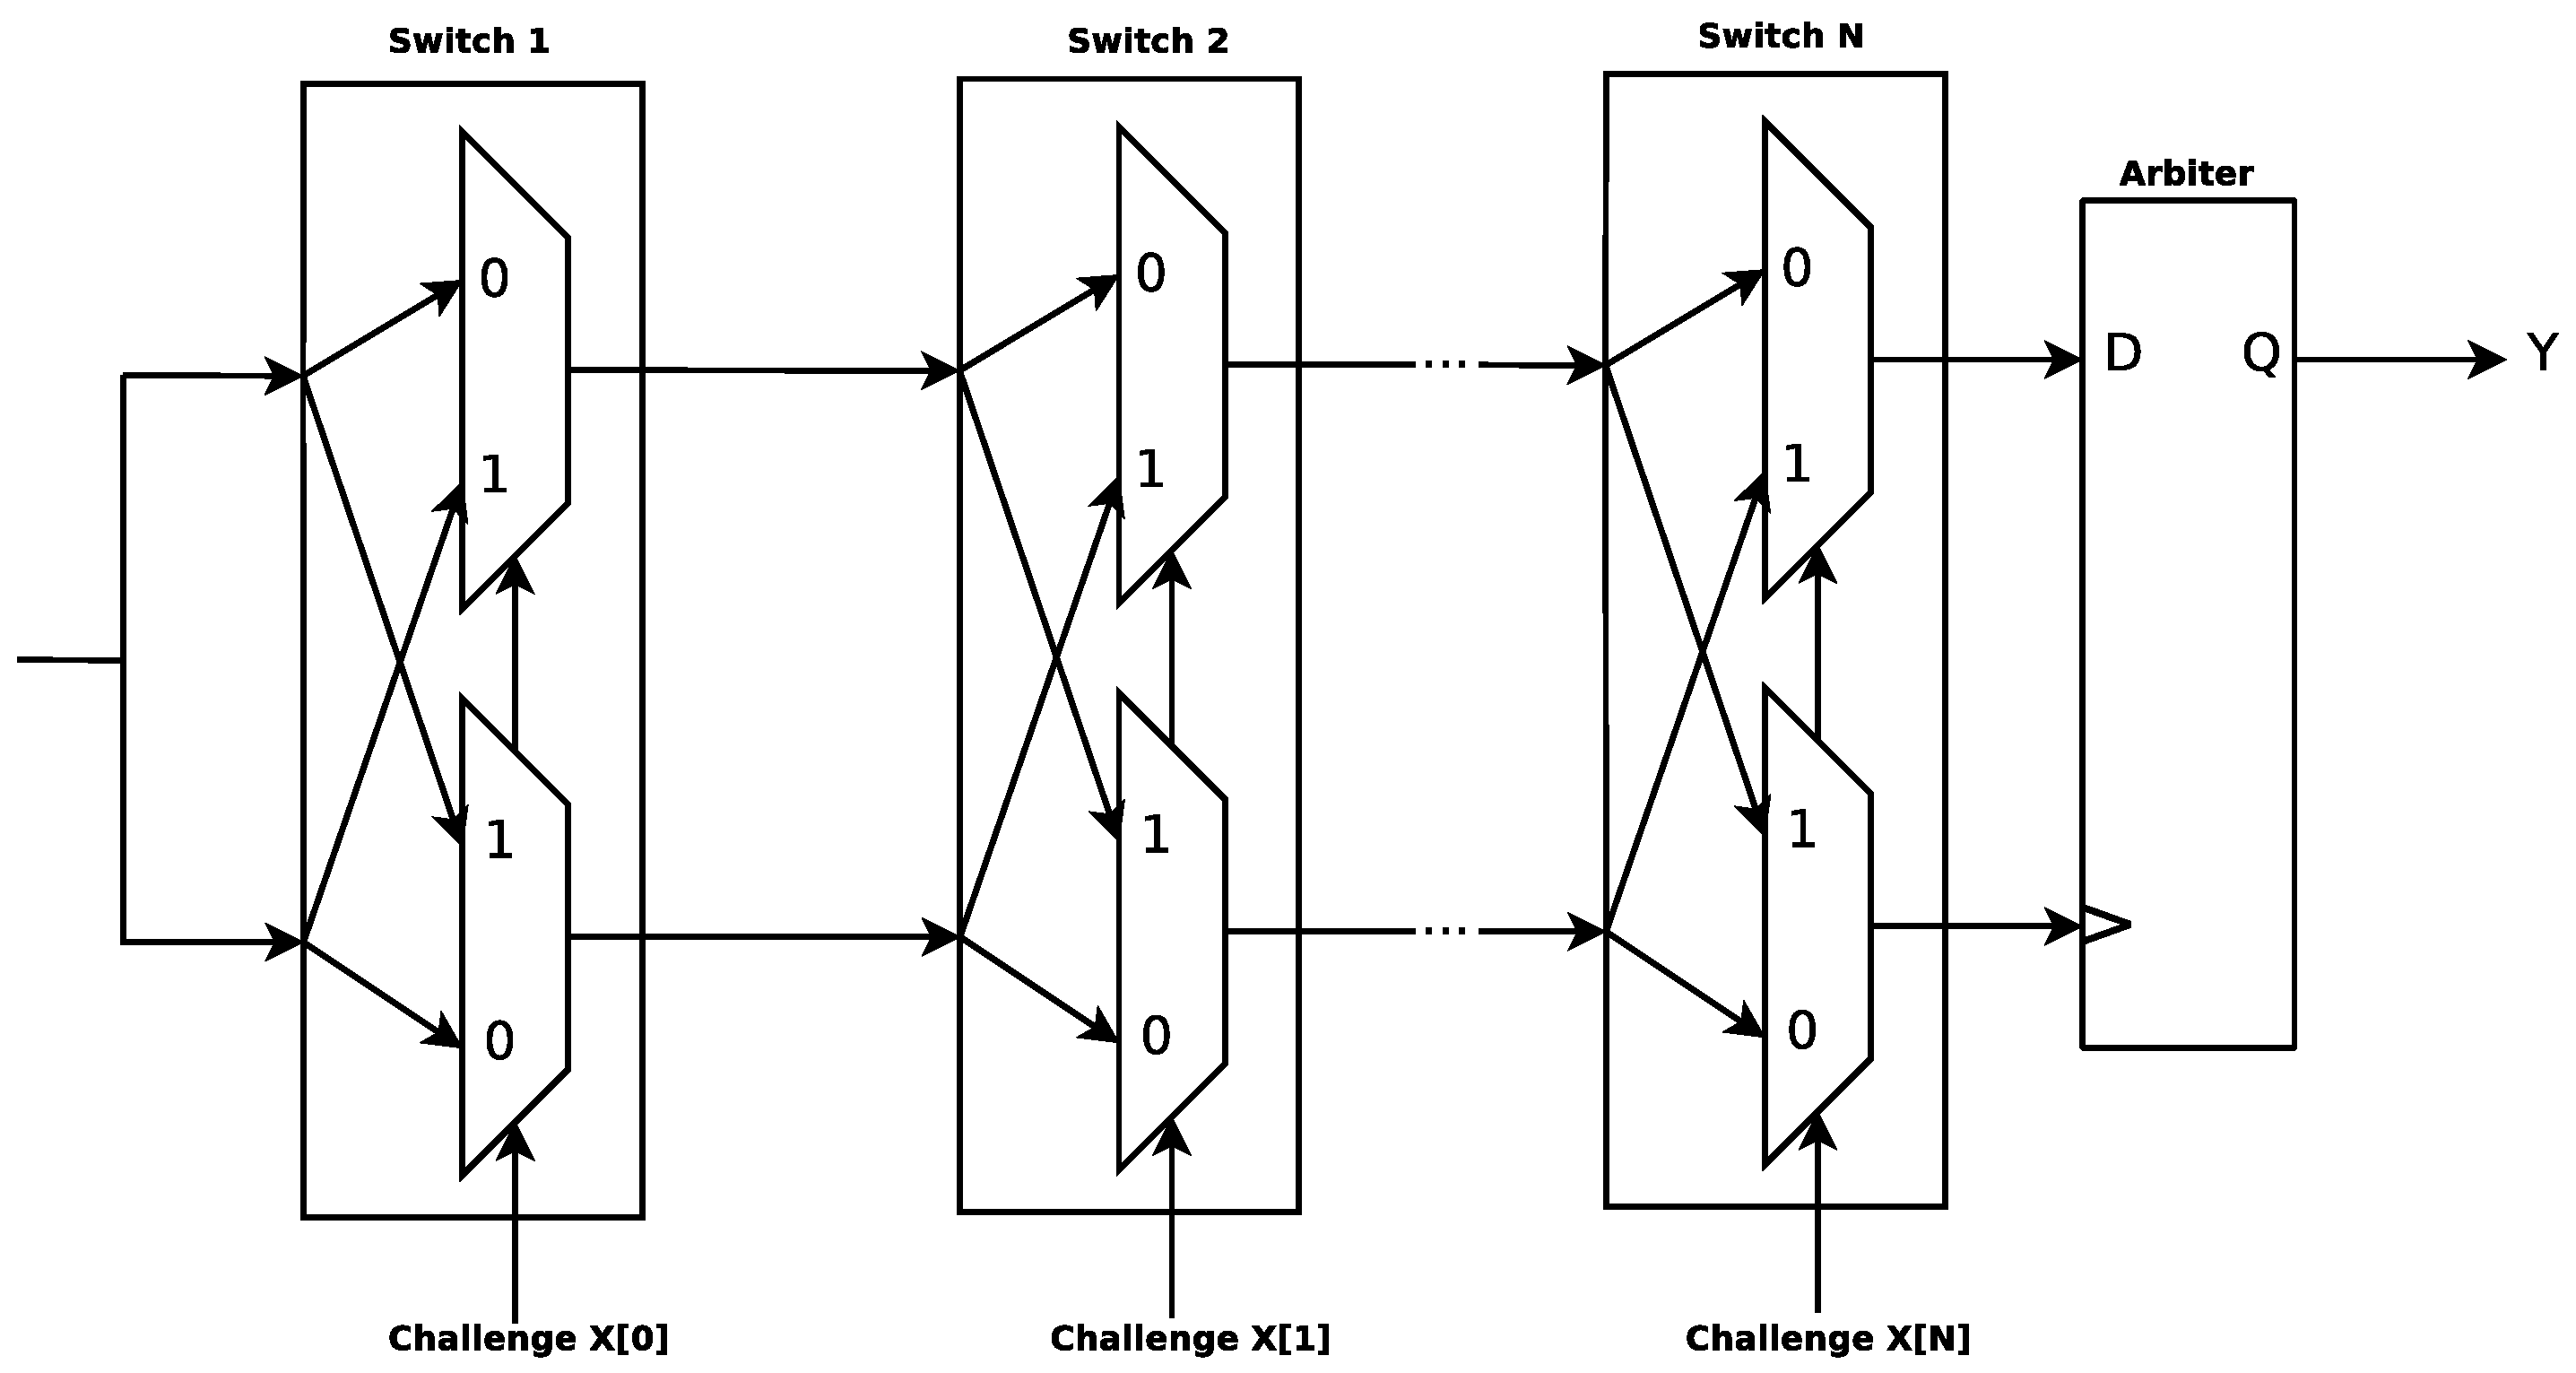
\includegraphics[width=0.85\textwidth]{arbiter}
	\caption{One arbiter \puf~ that receives a challenge $X$ and produces the output $Y$.}
%	\vspace*{-9pt} 
	\label{fig:arbiterpuf}
\end{figure*}

Another \puf~ type is the Static Random-Access Memory (SRAM) \puf~ \mario{Cite the author properly}\cite{Leest2012}, in this model, each SRAM cell within an SRAM block can be considered a \puf~. The typical cell implementation, shown in Figure \ref{fig:spufexample} is built from two cross-coupled inverters at its core, from an electronic viewpoint, this circuit contains a positive feedback loop which reinforces its current state. In a logic sense, this circuit has two stable values, and by residing in one of both states the cell stores one binary digit.%\mario{reduce the technical part and explain the concepts in a higher level}

The operation principle of an SRAM PUF is based on the transient behavior of an SRAM cell when it is powered up, i.e., when its supply voltage Vdd comes up. The circuit will evolve to one of its operating points, but it is not immediately clear to which one. In Figure   \ref{fig:spufexample} the inverters $I_1$ and $I_2$ have its drive strength determined by the process variations when this memory was manufactured, these inverters will compete to achieve stability. When one of the inverters is significantly stronger than the other one, the preferred initial operating point will be a stable state, and the preference will be very distinct, i.e., such a cell will always power-up in the same stable state, but which state this is (‘0’ or ‘1’), is randomly determined for every cell.
So in a \puf~ that uses an SRAM, the challenge is the row and column addresses, the output is the state of the cell after power up.
\begin{figure*}[!ht]
	\centering
	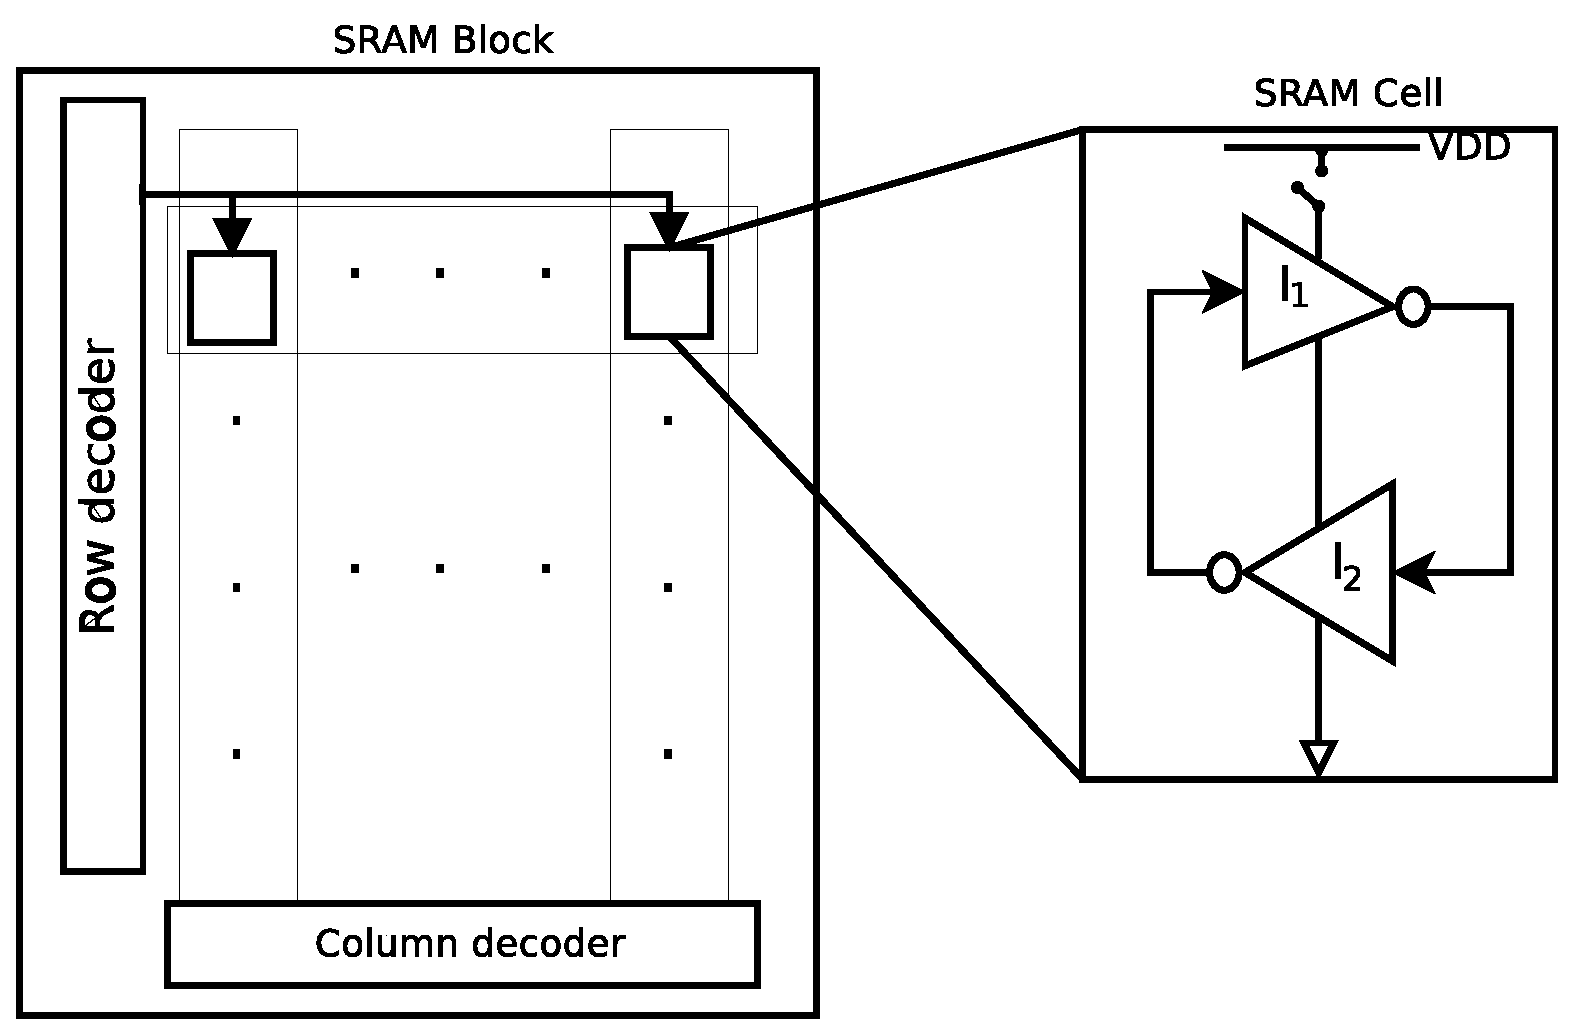
\includegraphics[scale=0.42]{figures/pdf/spuf}
% 	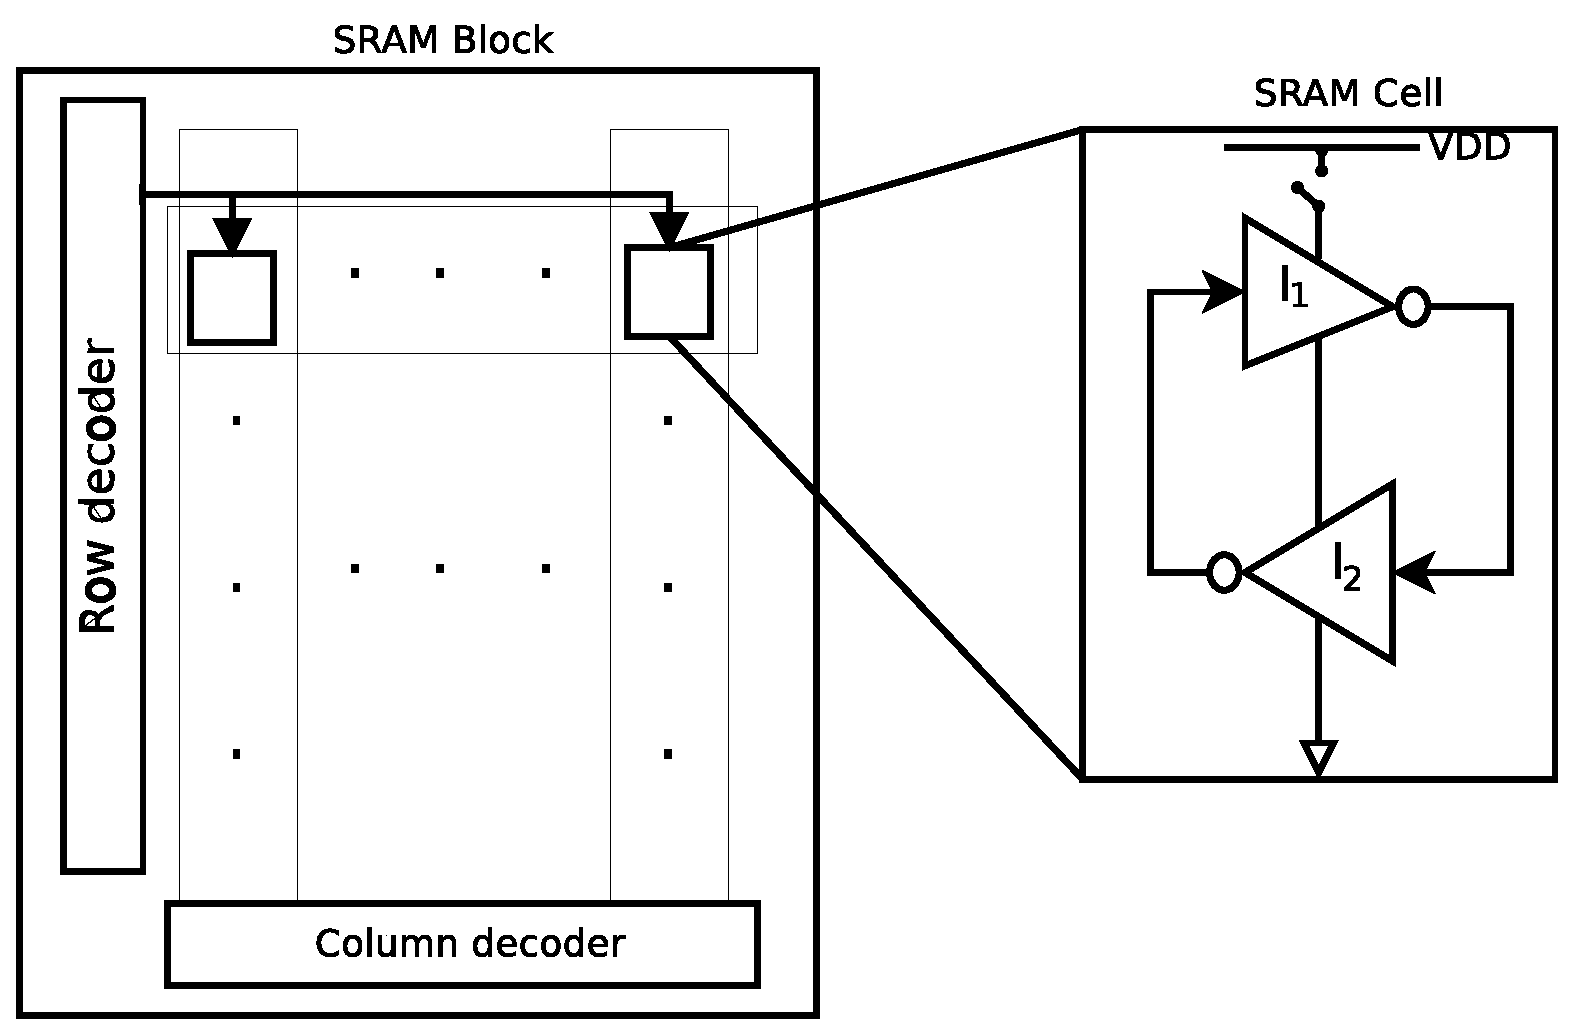
\includegraphics[width=\textwidth]{figures/pdf/spuf}
	\caption{A simplistic example of a SRAM \puf~ , showing the SRAM cell logic circuit inside an SRAM block.}
%	\vspace*{-9pt} 
	\label{fig:spufexample}
\end{figure*}


\subsection{\puf~ as a Cryptographic  Key Generator }
When a system needs a key in hardware for any purpose, such as encryption, authentication, or any other application, this key needs to be generated and stored in hardware \cite{puf-key-devadas-1278484}. The main advantage of using \pufs~as key generators is that they can produce keys at running time, this way, on-chip memories are not needed for key storage. Another benefit is that they are unclonable, meaning that even the manufacturer itself cannot produce two \puf~instances that will have the same set of Challenge-Response Pairs (\crps) \cite{Gassend2002:PUFs}. \mario {Better not to mix the work with the concepts}
\rem{\cshia~ uses a SRAM \puf~ together with a Fuzzy Extractor and the key extraction process is described in Section \ref{subsubsec:Key-Extraction}.}


%======================================================================
\section{Security Properties}
\label{sec:securityproperties}
In order to build a robust system, a designer has at his disposal mechanisms that implements three security properties: \mario{Briefly  introduce the concepts here and check the correct definition of each for instance : Preservation of confidentiality , integrity and availability of information, in addition other properties, such as authenticity, accountability, non-repudiation and reliability can also be involved (ISO/IEC 27000:2009)}authenticity, integrity, and secrecy. Although these features can be implemented through software, the stringent nature of embedded systems demands solutions that consume few clock cycles and are not power consuming.
In the following, we discuss hardware implementation of those security features.

%---------------------------------------------------------
\subsection{Authenticity}
\label{subsec:Authenticity}
Suppose that an attacker wants to add \hisher~own code for execution in the embedded system or intends to move the data from one system instance to another. These attacks can be avoided by employing authentication mechanisms. In this solution, a key (or unique set of keys) is determined for each instance.
%TODO explain the instance more clear
Code \andor~ data are tagged using these keys during manufacturing. \mario{this is typical of integrity } At run time, this key (or set of keys) is used to regenerate tags. Only a correct key value will be able to verify what was installed during manufacture. Therefore, an instance will not accept code or data that was not tagged using its own keys.

Before the introduction of electronic \pufs \cite{Gassend2002:PUFs}, these keys had to be inserted into the system before they were made available to the users. To do so, keys are stored on-chip using non-volatile memories and the manufacturer\slash{}vendor controlled the uniqueness of the keys in each instance. The main downsides of storing key permanently include: facilitating physical attacks \cite{Sadeghi2010:Security-PUFs}, and possibly increasing costs of production since it may demand integration of different technologies on the same chip.

%---------------------------------------------------------
\subsection{Integrity}
\label{subsec:integrity}
Similarly to authentication, integrity is ensured by tagging code and data with additional information such as memory address location \andor~timestamps. This prevents an attacker from tampering with a system by, for instance, moving instructions from their location in memory, setting different initial values of variables, etc. The level of integrity can be done for an entire program, memory pages, or memory blocks. 

Integrity can also be considered at the instruction sequence level, which we refer as Control-Flow Integrity (CFI). Hardware solutions for control-flow integrity usually require deep integration between hardware and software \cite{Davi2015:HAFIX}, that can result not only in changing the Instruction Set Architecture (\isa) \andor~the tool-chain, but also the processor's data path, as proposed in \cite{Gelbart2005:CODESSEAL, Kanuparthi2012:DynamicIntegrity}. Even though CFI protection is welcomed, many embedded system applications cannot afford the performance penalties and storage overhead inherently of this solution. For instance, in applications where user inputs are limited and \io~involves fixed amounts of data, an attacker has very little room to employ a buffer overflow or similar attacks prevented by CFI. However, integrity verification regarding blocks of code and data (as mentioned above) can avoid a variety of situations that go beyond run time attacks. For example, if an embedded system is unwatched, an attacker can upload malicious code or modify the data in the external memory even if the system is not running. Integrity verification can prevent and indicate these violations before they reach the processor.


%---------------------------------------------------------
\subsection{Secrecy}
\label{subsec:Secrecy}

An embedded system can also use encryption to prevent exposure of code \andor~data stored in the external memory. Consequently, the processor can run these instructions and data only after decryption. Therefore, the major drawback of using encryption is the performance overhead that highly depends on which cryptographic primitive is employed \cite{Suh2007:PUFs}. Also, secrecy only prevents that an attacker obtains the information, if it is not combined with a unique key or integrity verification, the system will be vulnerable to execute code of different system instances \andor~to suffer \mario{Explain attacks?} \ed{relocation and replay attacks\cite{Elbaz2009}.}

\mario{It is common to end each chapter with a closure,  in a higher abstraction level do a connections with  the next chapters }

\chapter{Related Work}
\label{chap:related_work}

\soc~devices have a number of features which distinguish them from other traditional electronic solutions. Their dedicated nature allows the adoption of more intrusive protection, while posing challenging energy and performance requirements. Unfortunately, traditional security solutions based on typical cryptographic mechanisms (e.g. bus encryption)  can have a significant impact in device cost, energy efficiency and performance. One way to go around that is to consider approaches which enable a deep integration of device hardware-intrinsic features and program execution, as those offered by \pufs.

Qualitative analyses of \pufs~have already been done in the literature~\cite{Katzenbeisser2012} motivated by several applications such as cryptographic key generation~\cite{Suh2007, Bhargava2014} and true random number generation~\cite{Leest2012, Herrewege2013}. Unlike those works, which aim at evaluating the quality of a standalone \puf-inspired mechanism, this work focus on proposing and analyzing a \puf-based micro-architecture mechanism to enable secure code execution. %\new{On big conundrum on using \pufs~is how to prevent unintended bit-flips on responses used to compound the cryptographic key. An approach to deal with that is to use post-processing schemes like Fuzzy Extractors \cite{}. Despite Fuzzy Extractors be a simple and known circuits, they the weakest spot on the architecture and can leak the cryptographic key through side channel attacks. }

Most of the preliminary work on secure code execution aimed at keeping instructions and data secure from scrutiny, by using mechanisms like bus encryption. In~\cite{Elbaz2005}, Elbaz \etal~performed a comprehensive survey of bus encryption, where they describe many possible ways of using cryptographic algorithms in \soc~architectures, so as to ensure that no malicious instruction\slash{}data would be executed by the CPU. The major shortcoming of these solutions is the usage of on-chip secret key storage in non-volatile memories which enable off-line key recovery attacks~\cite{towardshardwaresecurity2010}.

AEGIS, the secure processor proposed by Suh \etal~in~\cite{Suh2005}, employs \pufs~as a cryptography primitive to uniquely authenticate code and data in order to prevent both software and physical attacks. They present a toolchain for developing secure software for their architecture which includes a secure operating system to manage different levels of memory protection. Although the presented toolchain does not require modifications in the processor architecture, it demands extensive changes in the \soc~architecture, in addition to changes in the compiler and operating system. Moreover, AEGIS \emph{does not} ensure full-time security from power-on to power-off; i.e. the system runs unprotected until the security kernel loads the system. In addition, physical attacks were neither evaluated nor simulated. Different circuits used in AEGIS, like \pufs~and post-processing schemes for key extraction such as Fuzzy Extractors, have been successfully attacked with side-channel \cite{Merli2011,Tajik2016:Photonic} and semi-invasive attacks \cite{Tajik2015:LaserAttack}. While semi-invasive attacks are hard to repeal, side-channel attacks have few known countermeasures \cite{Merli2013:Masking} that can be easily adopted.



\chapter{CSHIA  Architecture}
\label{chap:cshia_architecture}



  %\system, illustrated in Figure \ref{fig:system}, is a processor architecture which aims at providing secure code execution by means of \puf-based authentication of cache lines. The central idea behind \system~is a \puf-Tag (\ptag) Memory, which runs in parallel with the system main memory (Figure \ref{fig:system}). Each entry in the \ptag~Memory stores an authentication code of a cache line generated by a \puf-based device located on-chip.
  
%   \begin{figure*}[!ht]
% 	\centering
% 	\includegraphics[scale=0.35]{cshia}
% %	\vspace*{-12pt} 
% 	\caption{A system overview of the \system~system.}
% %	\vspace*{-9pt} 
% 	\label{fig:system}
% \end{figure*}

  %\new{In comparison to traditional architectures, \system~includes two main modifications: The \textit{Secure Engine} (\tagsystem), which includes the \textit{PTAG Generator} (\ptaggen, Figure \ref{fig:ptaggen}); and the \textit{Security-Cache} (\seccache) that controls bus traffic between the processor and the \textit{Memory Controller} (\mctrl). Other two new architectural components are also required to complete the \system~design, the \textit{\ptag~Memory} and the \textit{PTAG Bus}. In a few words, when the processor requires\slash{}sends data\slash{}instructions to the \mctrl, the \seccache~sends the related cache line to the \tagsystem~for computing\slash{}validating its \ptag. Notice from Figure \ref{fig:system} that the \ptag~bus runs in parallel to the system buses, and thus no program can directly read the \ptag~Memory, since neither the processor nor the \mctrl~are aware about the \seccache.}


  % \subsection{\ptaggen~Operation}
  % \label{subsec:ptaggenOpr}

  % \new{The \tagsystem~controls the \ptaggen~based on the information delivered by the \seccache. This information is generated from bus transactions (Memory READ, Memory WRITE and I\slash{}O) between the processor and the memory controller, and which the \seccache~controls. Next, each \ptaggen~action is explained in regard to bus transactions.}
  
  %     \begin{figure*}[!ht]
	 %  \centering
	 %  \includegraphics[scale=0.4]{ptaggen}
	 %  \caption{The \ptaggen~during \ptag~Generation (write) and \ptag~Verification (read) operations.}
  % %	\vspace*{-9pt} 
	 %  \label{fig:ptaggen}
  % \end{figure*}
  

	 %  \subsubsection{\ptag~Generation (memory write)}
	 %  \label{subsubsec:ptag-generation}
  % \new{During a write operation, the \seccache~passes data\slash{}instruction cache lines to the \tagsystem~and the \ptaggen~computes \ptags~and stores it into the \ptag~Memory. A \textit{Pseudorandom Function} (\prf) \cite{Goldreich2004} module is used to generate the \ptag~and takes as input the concatenation ($||$) of the cache line bits and the base address of the cache line provided by the core (see Figure \ref{fig:ptaggen}). In order to ensure uniqueness, the \prf~is configured using a \textit{unique-per-device key}. This key is produced by the intrinsic hardware features of a~\puf. Such authentication tag is specific to the core running that specific cache line, as ~\puf~outputs are dependent on the statistical variations of the manufacturing process, and are unique to each processor~\cite{Katzenbeisser2012}. Hence identical cache lines running on different processors will produce different \ptag~values for the same inputs. Notice that only code in the cache, for which integrity has been ensured, will be able to write to memory.}
  


	 %  \subsubsection{\ptag~Verification (memory read)}
	 %  \label{subsubsec:ptag-verification}
  % \new{During a read operation, the \seccache~passes data\slash{}instruction cache lines to the \tagsystem~and the \ptaggen~computes \ptags~for verification. As shown in Figure~\ref{fig:ptaggen}, during a read operation the cache line base address produced by the core is appended to the cache line contents read from memory and the result is fed to the \prf~module. The \ptag~produced this way is compared to the PTAG read from memory for equality. If the previously stored \ptag~and the recently computed value do not match, a \textit{Non-Maskable Interrupt} (NMI) is generated to the core (called \ptagnmi), as code\slash{}data integrity may have been violated. As shown in Figure \ref{fig:system}, in order to hide \puf~latency, the data\slash{}instruction is sent to the respective cache (I\$ or D\$) at the same time that \ptag-GEN computes the \ptag~for that cache line and compares it to its \ptag~previously stored into the \ptag~Memory.}

	 %  \subsubsection{Handling I\slash{}O}
	 %  \label{subsubsec:io}
  % In modern computer systems, I\slash{}O operations store data directly into specific memory regions through DMA mechanism. Thus, it is not possible to trust such memory regions and \system~does not ensure their integrity and authenticity. Software should first perform authentication of I\slash{}O data in a higher abstraction layer and then copy it to secure areas where the \system~can ensure integrity and authenticity.


\begin{figure*}[!ht]
	\centering
% 	\includegraphics[scale=0.45]{cshia}
	\includegraphics[width=\textwidth]{cshia}
	\caption{The \cshia~architecture.}
%	\vspace*{-9pt} 
	\label{fig:cshia}
\end{figure*}

\cshia~was originally proposed in \cite{Hoffman2015} as an architecture for \iot. However, we believe that \cshia~fits in a broader class of embedded system applications that can benefit from its nice security features. As we stated before, many embedded system applications do not need secrecy\slash{}confidentiality, but strongly require code and data authenticity and integrity. 
Using the original work with some architectural elements modified to provide stronger security features, the first LEON3 \fpga~ based implementation of \cshia was realized. This section focus on presenting our \cshia~implementation components and how they work to provide authenticity and integrity. Figure \ref{fig:cshia} illustrates the basic components required for \cshia~ to work: 
\begin{itemize}
    \item One core that in this implementation is a LEON3 processor;
    \item The \cshia~ components:
    \begin{itemize}
        \item \ptag~ Memory Management Unit (\pmmu)
        \item Bus Handler (\handler)
        \item Security Engine (\seceng) 
    \end{itemize}
    \item One external memory that contains instructions and data;
    \item One interconnection bus using AMBA2.
\end{itemize} 

\section{LEON3}

\section{AMBA2}
\begin{figure}[ht]
    \centering
    \includegraphics[width=1\textwidth]{figures/others/typica_ahb.png}
    \caption{Typical AMBA2 system , with a CPU , DMA and other low bandwidth peripherals }
    \label{fig:general}
\end{figure}

The BUS used in the LEON3 processor is the Advanced High-performance Bus (AHB), where on-chip memory and other Direct Memory Access (DMA) devices also reside. This bus provides a high-bandwidth interface between the elements that are involved in the majority of transfers. Also located on the high-performance bus is a bridge to the lower bandwidth APB, where most of the peripheral devices in the system are located. Figure \ref{fig:general} exemplify a traditional AHB utilization.


AMBA AHB implements the features required for high-performance, high clock
frequency systems including:
\begin{itemize}
 \item {burst transfers}
\item {split transactions}
\item {single-cycle bus master handover}
\item {non-tristate implementation}
\item {wider data bus configurations (64/128 bits).}
\end{itemize}

 
\subsection{AMBA AHB operation}

\begin{figure}[ht]
    \centering
    \includegraphics[width=0.7\textwidth]{figures/others/multiplex.png}
    \caption{Overview  of the AMBA2 Organization, with the arbiters masters and slaves distribution}
    \label{fig:internorg}
\end{figure}
The previously described AMBA components are seen by the bus as masters and slaves, as depicted in Figure \ref{fig:internorg}, where, for instance, the CPU is an AMBA master and on-chip RAM is a slave. Who decides the priorities and decode all access  is the AMBA arbiter, which will be described further.

Before an AMBA AHB transfer can commence the bus master must be granted access to the bus. This process is started by the master asserting a request signal to the arbiter. Then the arbiter indicates when the master will be granted use of the bus. A granted bus master starts an AMBA AHB transfer by driving the address and control signals. These signals provide information on the address, direction and width of the transfer, as well as an indication if the transfer forms part of a burst. Two different forms of burst transfers are allowed:
\begin{itemize}
\item incremental bursts, which do not wrap at address boundaries
\item wrapping bursts, which wrap at particular address boundaries.
\end{itemize}

A write data bus is used to move data from the master to a slave, while a read data bus
is used to move data from a slave to the master.
Every transfer consists of:

\begin{itemize}
\item an address and control cycle
\item one or more cycles for the data.
\end{itemize}

\begin{figure}[ht]
    \centering
    \includegraphics[width=0.4\textwidth]{figures/others/simple_ahb_transfer.png}
    \caption{AHB basic transfer with one cycle for address and control and one or many for data.}
    \label{fig:basic_ahb_transfer}
\end{figure}


The address cannot be extended and therefore all slaves must sample the address during this time. The data, however, can be extended using the HREADY signal. When LOW this signal causes wait states to be inserted into the transfer and allows extra time for the slave to provide or sample data, as can be seen in Figure \ref{fig:basic_ahb_transfer}. During a transfer the slave shows the status using the response signals, HRESP[1:0]:
\begin{itemize}

\item  {OKAY -} The OKAY response is used to indicate that the transfer is progressing normally and when HREADY goes HIGH this shows the transfer has completed successfully.
\item {ERROR -} The ERROR response indicates that a transfer error has occurred and the transfer has been unsuccessful.
\item {RETRY and SPLIT  -} Both the RETRY and SPLIT transfer responses indicate that the transfer cannot complete immediately, but the bus master should continue to attempt the transfer. In normal operation a master is allowed to complete all the transfers in a particular burst before the arbiter grants another master access to the bus. However, in order to avoid excessive arbitration latencies it is possible for the arbiter to break up a burst and in such cases the master must re-arbitrate for the bus in order to complete the remaining transfers in the burst.
\end{itemize}


\subsection{AMBA Components}
\augusto{say that we are reducing the scope to what was used in the design }
\subsubsection{Masters}
\begin{figure}[ht]
    \centering
    \includegraphics[width=0.7\textwidth]{figures/others/master_ahb.png}
    \caption{AHB master interface}
    \label{fig:masterint}
\end{figure}

 An AHB bus master has the most complex bus interface in an AMBA system , its interfaces are depicted in Figure \ref{fig:masterint}. Typically an AMBA system designer would use predesigned bus masters and therefore would not need to be concerned with the detail of the bus master interface.



\subsubsection{Slaves}

\begin{figure}[ht]
    \centering
    \includegraphics[width=0.7\textwidth]{figures/others/slave_ahb.png}
    \caption{AHB slave interface}
    \label{fig:slaveint}
\end{figure}
An AHB bus slave(\ref{fig:slaveint}) responds to transfers initiated by bus masters within the system. The slave uses a HSELx select signal from the decoder to determine when it should respond to a bus transfer. All other signals required for the transfer, such as the address and control information, will be generated by the bus master.
 
\subsubsection{Arbiter}
\begin{figure}[ht]
    \centering
    \includegraphics[width=0.7\textwidth]{figures/others/arbiter_ahb.png}
    \caption{AHB arbiter interface}
    \label{fig:arbiterint}
\end{figure}
 The role of the arbiter in an AMBA system is to control which master has access to the bus. As can be seen in Figure \ref{fig:arbiterint} every bus master has a REQUEST / GRANT interface to the arbiter and the arbiter uses a prioritization scheme to decide which bus master is currently the highest priority master requesting the bus. Each master also generates an HLOCKx signal which is used to indicate that the master requires exclusive access to the bus. The detail of the priority scheme is not specified and is defined for each application. It is acceptable for the arbiter to use other signals, either AMBA or non-AMBA, to influence the priority scheme that is in use.

 
\subsubsection{Arbitration}
 The arbitration Process  need specific control signals described  below:
 \begin{itemize}
\item  {\textbf{HBUSREQx -}} The bus request signal is used by a bus master to request access to the bus. Each bus master has its own HBUSREQx signal to the arbiter and there can be up to 16 separate bus masters in any system.
\item  {\textbf{HLOCKx -}} The lock signal is asserted by a master at the same time as the bus request signal. This indicates to the arbiter that the master is performing a number of indivisible transfers and the arbiter must not grant any other bus master access to the bus once the first transfer of the locked transfers has commenced. HLOCKx must be asserted at least a cycle before the address to which it refers, in order to prevent the arbiter from changing the grant signals.
\item  {\textbf{HGRANTx -}} The grant signal is generated by the arbiter and indicates that the appropriate master is currently the highest priority master requesting the bus, taking into account locked transfers and SPLIT transfers.
A master gains ownership of the address bus when HGRANTx is HIGH and HREADY is HIGH at the rising edge of HCLK.
\item  {\textbf{HMASTER[3:0] -}} The arbiter indicates which master is currently granted the bus using the HMASTER[3:0] signals and this can be used to control the central address and control multiplexor. The master number is also required by SPLIT-capable slaves so that they can indicate to the arbiter which master is able to complete a SPLIT transaction.
\item  {\textbf{HMASTLOCK -}} The arbiter indicates that the current transfer is part of a locked sequence by asserting the HMASTLOCK signal, which has the same timing as the address and control signals.

\item  {\textbf{HSPLIT[15:0] -}} The 16-bit Split Complete bus is used by a SPLIT-capable slave to indicate which bus master can complete a SPLIT transaction. This information is needed by the arbiter so that it can grant the master access to the bus to complete the transfer.
\end{itemize}

An Example of a master requesting the bus control is shown in Figure \ref{fig:grantwait} where the arbiter grants the access after a few waiting cycles.
 \begin{figure}[ht]
    \centering
    \includegraphics[width=\textwidth]{figures/others/arbiter_grant_wait.png}
    \caption{Granting with wait cycles}
    \label{fig:grantwait}
\end{figure}


\subsubsection{Decoder}
\begin{figure}[ht]
    \centering
    \includegraphics[width=0.7\textwidth]{figures/others/decoder_ahb.png}
    \caption{AHB Decoder interface}
    \label{fig:decoder int}
\end{figure}
 The decoder in an AMBA system is used to perform a centralized address decoding function, which improves the portability of peripherals, by making them independent of the system memory map.

 



\section{\cshia~Components}
\label{sec:Components-of-the-Architecture}
As Section \ref{subsec:integrity} discussed, the main resource to provide integrity are tags. Since \cshia~uses \puf-based keys to generate tags, we called them \puf-Tags, or \ptags~for short. \ptags~are the core of \cshia's design. They will be unique for each instance of \cshia~due to the unclonability property of \pufs. That ensures one-to-one relationship between programs and instances, providing authenticity. To handle \ptags, three main components are added to a conventional embedded system architecture. They are: The \ptag~Memory; the Bus Handler (\handler); and the Security Engine (\seceng). Figure \ref{fig:cshia} shows this design and how components communicate between themselves. 

\ptag~Memory is an external memory and has its own buses. This architectural decision gives freedom to designers that can choose bus width, frequency, address space, etc. Because the processor is not aware of any additional component of \cshia, \handler~intercepts data transfers between processor and memory in order to provide them to \seceng~that generates tags. \handler~can also request data ( on behalf of the processor) to main memory so as  form complete memory blocks that are necessary to generate \ptags.

\seceng~has three major sub-components. The main one is the \ptag~Generator (\ptaggen), which uses input data whose length is equal to a memory block concatenated with its address to generate \ptags. The \fuzzy~is only used when the system loses its secret key. For instance, after a power cycle. Thus, when the system is powered on, the \fuzzy~will extract the \puf-based key and provide it to \ptaggen. Finally, we have the \ptag~Memory Management Unit (\pmmu). The main functions of the \pmmu~are to store and request \ptags~from the \ptagmem~and also to decode internal addresses of \ptags~to physical addresses of \ptagmem. 


%======================================================
%Security Handler
%======================================================
\subsection{Bus Handler (\handler)}
This block has three main functions, monitoring the processor requests and respond then when necessary, 
assemble a line %explain better what line means
that can be multiple cache lines or any other combination necessary to be in the format
 of the security engine input  and prevent the processor the execute unsafe or unverified instructions
 as well as don't let  it  write in the bus any unsafe operation.
%======================================================
%Block Diagram
%======================================================
\subsubsection{Block Diagram}

\begin{figure*}[!ht]
	\centering
	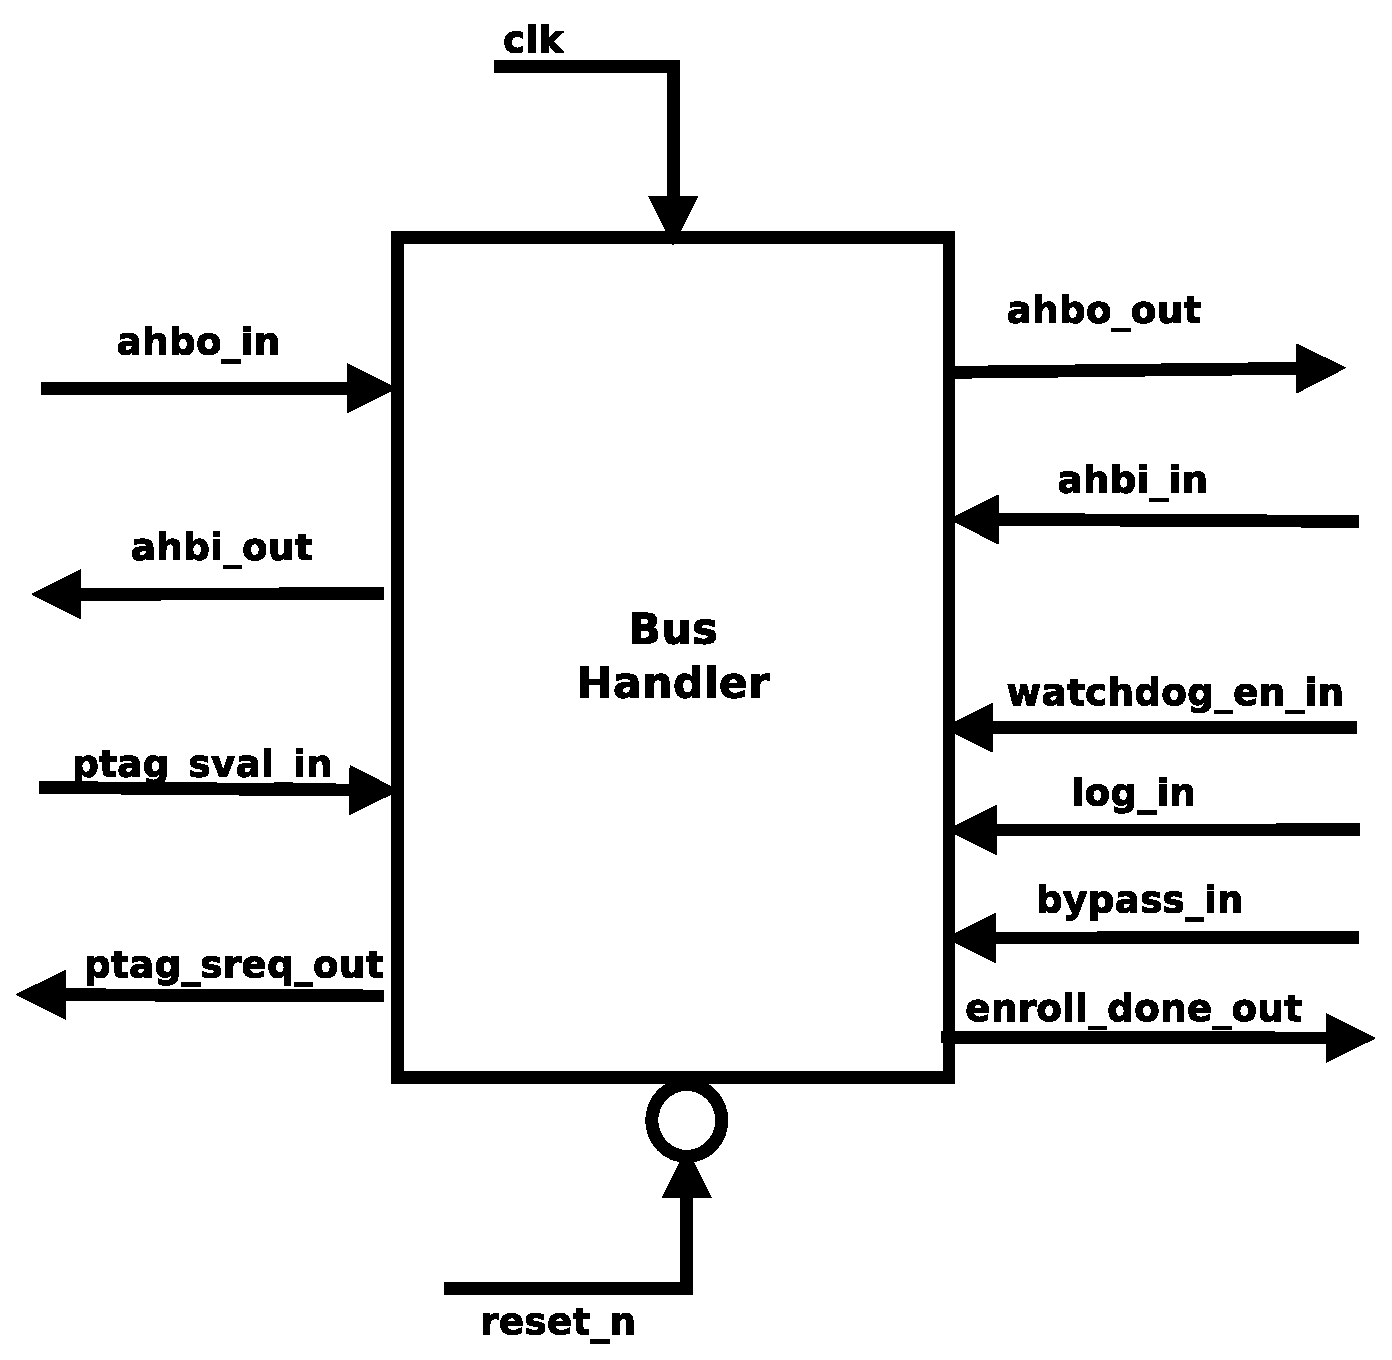
\includegraphics[scale=0.35]{bus_handler}
    \caption{Bus Handler  black box  }
%	\vspace*{-9pt} 
	\label{fig:bhbb}
\end{figure*}


%======================================================
%Signal Description
%======================================================
\subsubsection{Signal Description}

The inputs and outputs of this block can be split in three interfaces and control being
the signals  ahbo\_in and ahbi\_out the interface with the LEON3 processor,  ahbo\_out  and ahbi\_in
the interface with the bus , ptag\_sval\_in and ptag\_sreq\_out with the security engine  and control
 the signals clk ,reset\_n and bypass\_in.
 The description of each type can be found in the Appendix \ref{ap:signals}.
\begin{table}[H]
\centering
\label{table:shports}
\begin{tabular}{l l l l}
\textbf{Port}   & \textbf{in/out} & \textbf{Type}        & \textbf{Description} 	\\ \hline \hline
clk             & in              & std\_ulogic          & system clock         	\\ \hline
rstn            & in              & std\_logic           & negated rset         	\\ \hline
bypass\_in      & out             & std\_logic           & bypass input         	\\ \hline
ptag\_sreq\_out & out             & ptag\_sec\_req\_type & security check request    	\\ \hline
ptag\_sval\_in  & in              & ptag\_sec\_val\_type & security check response  	\\ \hline
ahbi\_in        & in              & ahb\_mst\_in\_type   & AHB input from bus      	\\ \hline
ahbi\_out       & out             & ahb\_mst\_in\_type   & AHB output to processor      \\ \hline
ahbo\_in        & in              & ahb\_mst\_out\_type  & AHB input from processor    \\ \hline
ahbo\_out       & out             & ahb\_mst\_out\_type  & AHB output to BUS            \\ \hline
\end{tabular}
 \caption{Ports of the security handler}
\end{table}





\subsubsection{Functional Description}


\begin{figure*}[!ht]
	\centering
	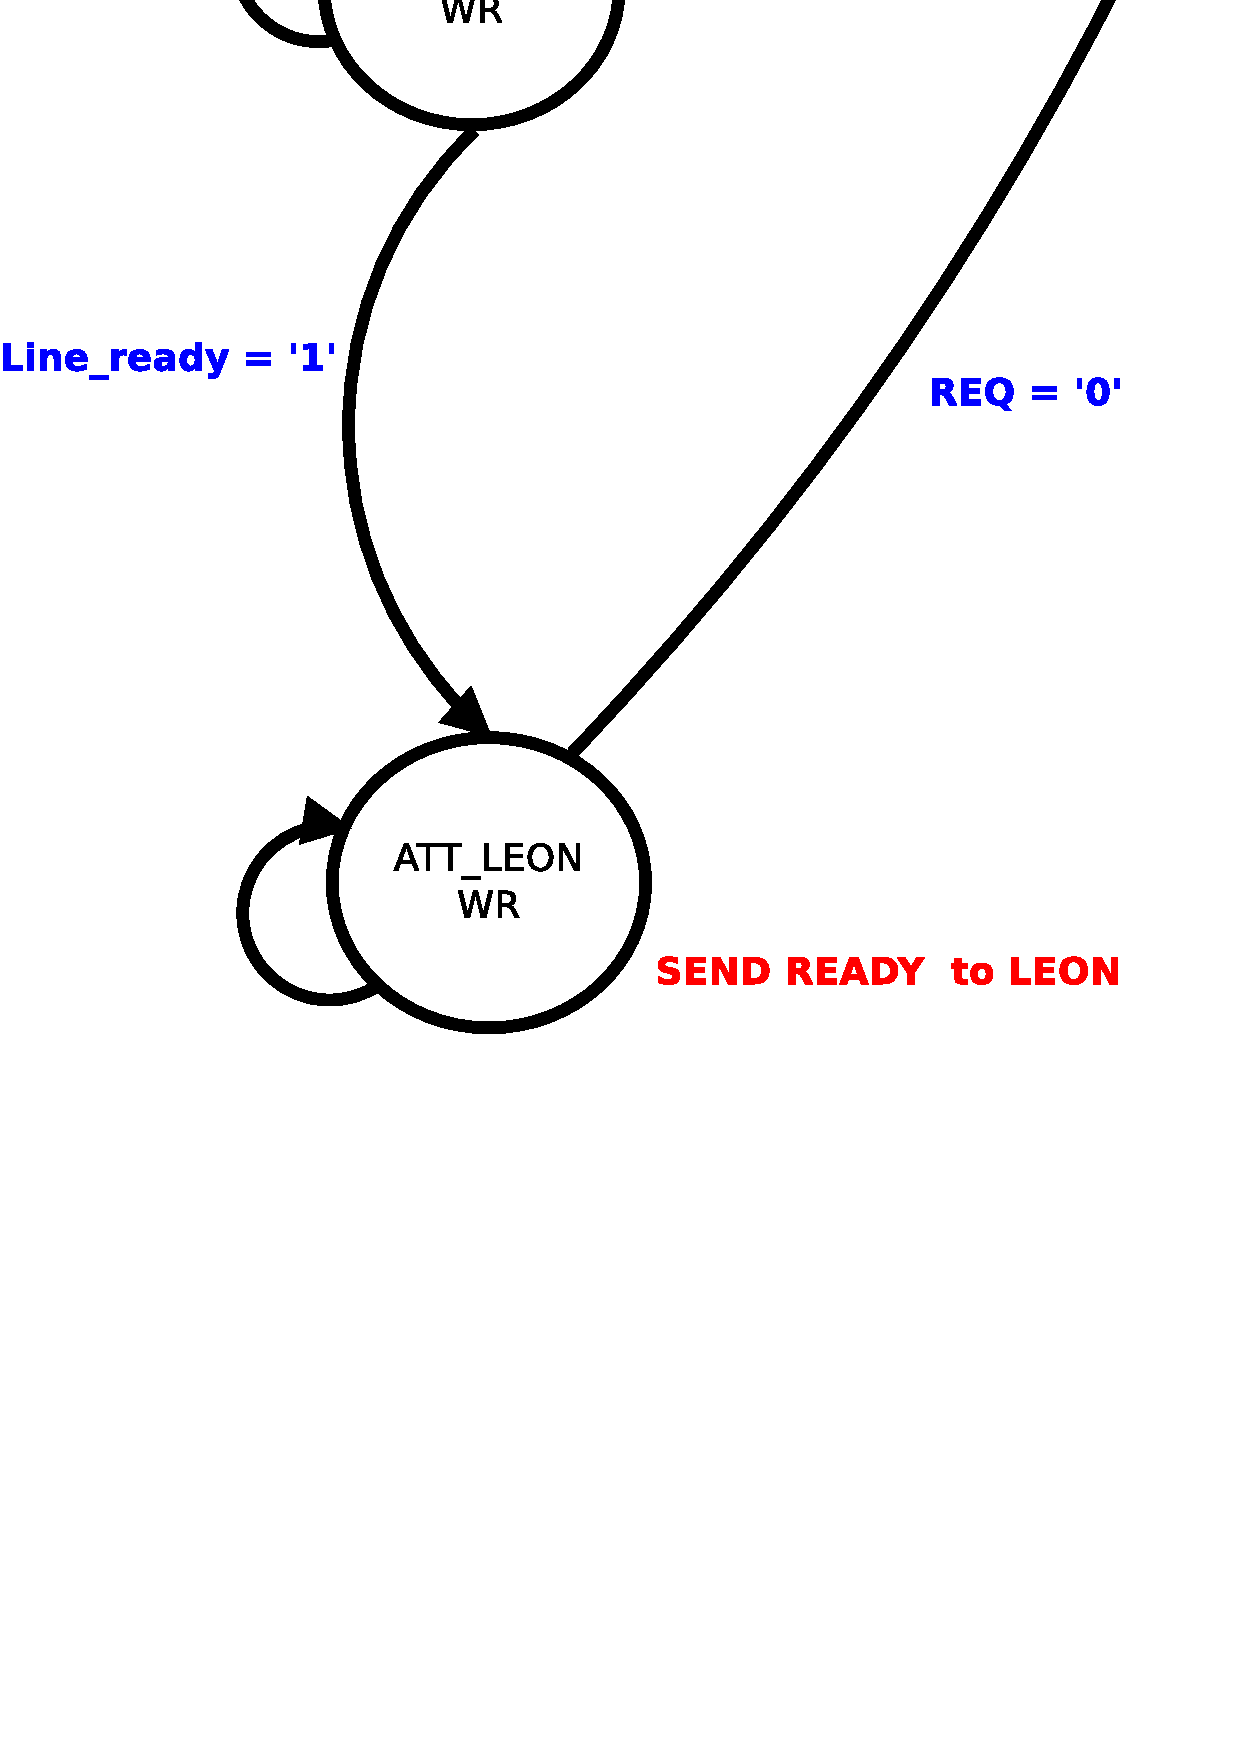
\includegraphics[scale=0.25]{figures/pdf/state_machine_force.pdf}
    \caption{Bus Handler state machine  }
%	\vspace*{-9pt} 
	\label{fig:phsm}
\end{figure*}
Since this  state machine controls all the operations of the security handler the functional 
description of this block can be explained using the state transactions of Figure \ref{fig:phsm} and the 
following state description:

\begin{itemize}
 \item{\textbf{IDLE}}
 
 The system stay in this state  until the processor signalizes a request, given the request 
 there are three options, the line contains the content requested by the processor, in this case
 the request can be responded in the SERVE LEON state, the line does not contain the content required
 so a new line must be loaded in the READ GRANT state or the current line is not safe and the system will halt
 going to UNSAFE state.
 
  \item{\textbf{READ GRANT}}
  
  This state is required for any transaction in the bus, it requests the bus grant for the arbiter prior to 
  begin the request, once the arbiter gives the grant the line status is checked and if the line is dirty( the processor
  update any value in the line) then it needs to be written in the memory before loading a new line, if this is the case
   then the system goes to WRITE LINE state, if no changes were made in the line then a new line is loaded in the READ LINE 
   state. The steps needed to acquire the bus grant are shown in section \ref{op:grant}.
  
  \item{\textbf{READ LINE}}
  
  
  A new line will be loaded from the main memory to the local buffer,the  steps needed to execute
   a read or write operation is shown  in \ref{op:rw}, so a counter is started and counts the 
  number of words the bus provided, so when the line is loaded the line status is changed to valid and
  the system goes back to IDLE state. When  the line is ready  then a request is sent to the security engine 
  to check if the line is safe and the system will freeze until the integrity of the line is confirmed.

 \item{\textbf{WRITE LINE}}
 
 Once the line is dirty and need to be written in the main memory, a counter is  started, similar to the read process 
 but it now counts each time the write request is confirmed by the bus, when all words were written  the line dirty status 
 is now changed to not dirty and the system goes to IDLE. In the process of writing the line to memory, in parallel a request is made 
 to the security engine to calculated the new PTAG related to its line and store it in the PTAG memory.

 \item{\textbf{SERVE LEON}}

 On this state  all LEON requests  read or write are executed, if the content needed is  in the line. 
 when any operation requires a word  that is not in the local line buffer then the system  goes back to IDLE state.
 
 
 \item{\textbf{UNSAFE}}
 
 
When a security check fails  on the IDLE state the system uses this as a trap state to halt.

\end{itemize}




\subsubsection{Bus Operations}

\begin{subsubsection}{Requesting Grant}
\label{op:grant}


  \begin{figure}[H]
    \centering
    \includegraphics[width=0.95\textwidth]{figures/others/grant_nowait.png}
    \caption{Requesting grant with no wait states  }
    \label{fig:gnwsm}
\end{figure}


  \begin{figure}[H]
    \centering
    \includegraphics[width=0.95\textwidth]{figures/others/grant_wait.png}
    \caption{Requesting grant with wait states  }
    \label{fig:gwsm}
\end{figure}
\end{subsubsection}

\begin{subsubsection}{Read and Write BUS Operations}
\label{op:rw}


  \begin{figure}[H]
    \centering
    \includegraphics[width=0.95\textwidth]{figures/others/undef_burst_length.png}
    \caption{burst transfer with undefined lengths read and write }
    \label{fig:ublsm}
\end{figure}

\end{subsubsection}






%======================================================
%Security Engine
%======================================================
\subsection{Security Engine}

This block is responsible for the interface with the external memory which stores the physical tags values
for each sets of challenges, and for calculating this values using one or more \pufs~, the \puf~ description is in Section \ref{subsec:Enrollment-Phase}.


\begin{figure*}[!ht]
	\centering
	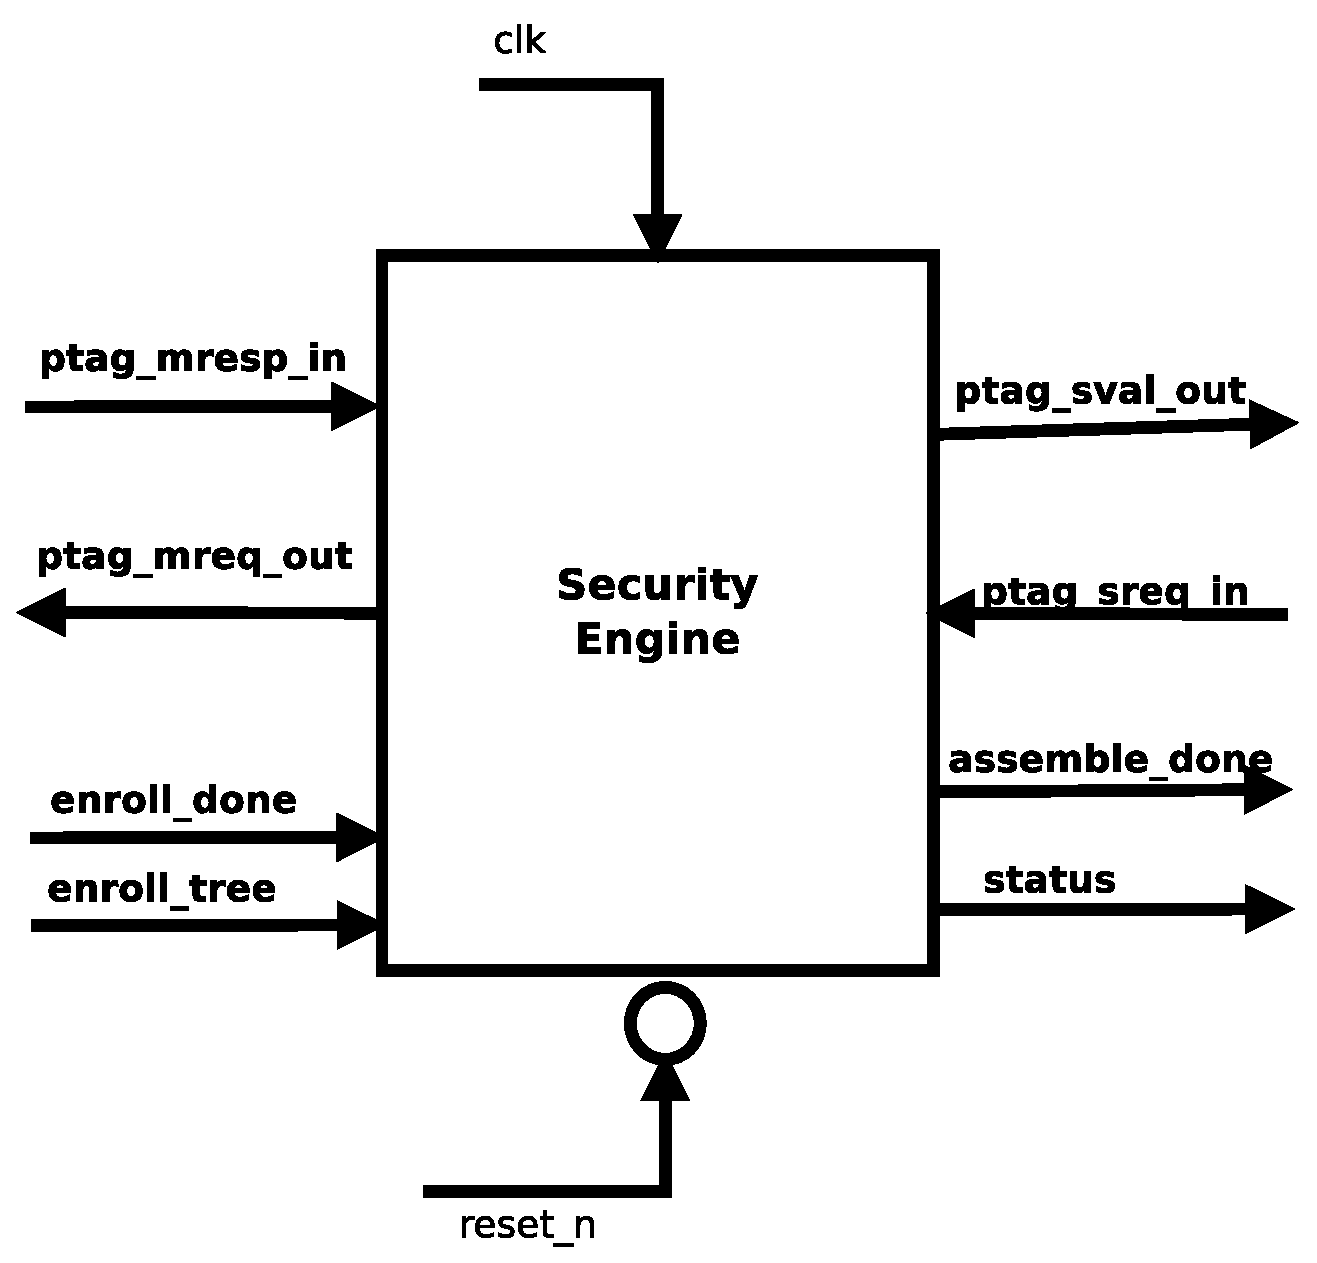
\includegraphics[scale=0.35]{security_engine_bb}
    \caption{Security engine  black box  }
%	\vspace*{-9pt} 
	\label{fig:sebb}
\end{figure*}




\subsubsection{Signal Description}

\begin{table}[H]
\centering
\label{table:seports}
\begin{tabular}{l l l l}

\textbf{Port}   & \textbf{in/out} & \textbf{Type}        & \textbf{Description} 	\\ \hline \hline
clk             & in              & std\_ulogic          & system clock         	\\ \hline
rstn            & in              & std\_logic           & negated reset         	\\ \hline
ptag\_sreq\_in  & in              & ptag\_sec\_req\_type & security check request    	\\ \hline
ptag\_sval\_out & out             & ptag\_sec\_val\_type & security check response  	\\ \hline
ptag\_mreq\_out & out             & ptag\_mreq\_type 	 & ptag memory  request    	\\ \hline
ptag\_mresp\_in & in              & ptag\_mresp\_type 	 & ptag memory  response  	\\ \hline
\end{tabular}
 \caption{Ports of the security engine}
\end{table}




\subsubsection{Functional Description}
  \begin{figure}[H]
    \centering
    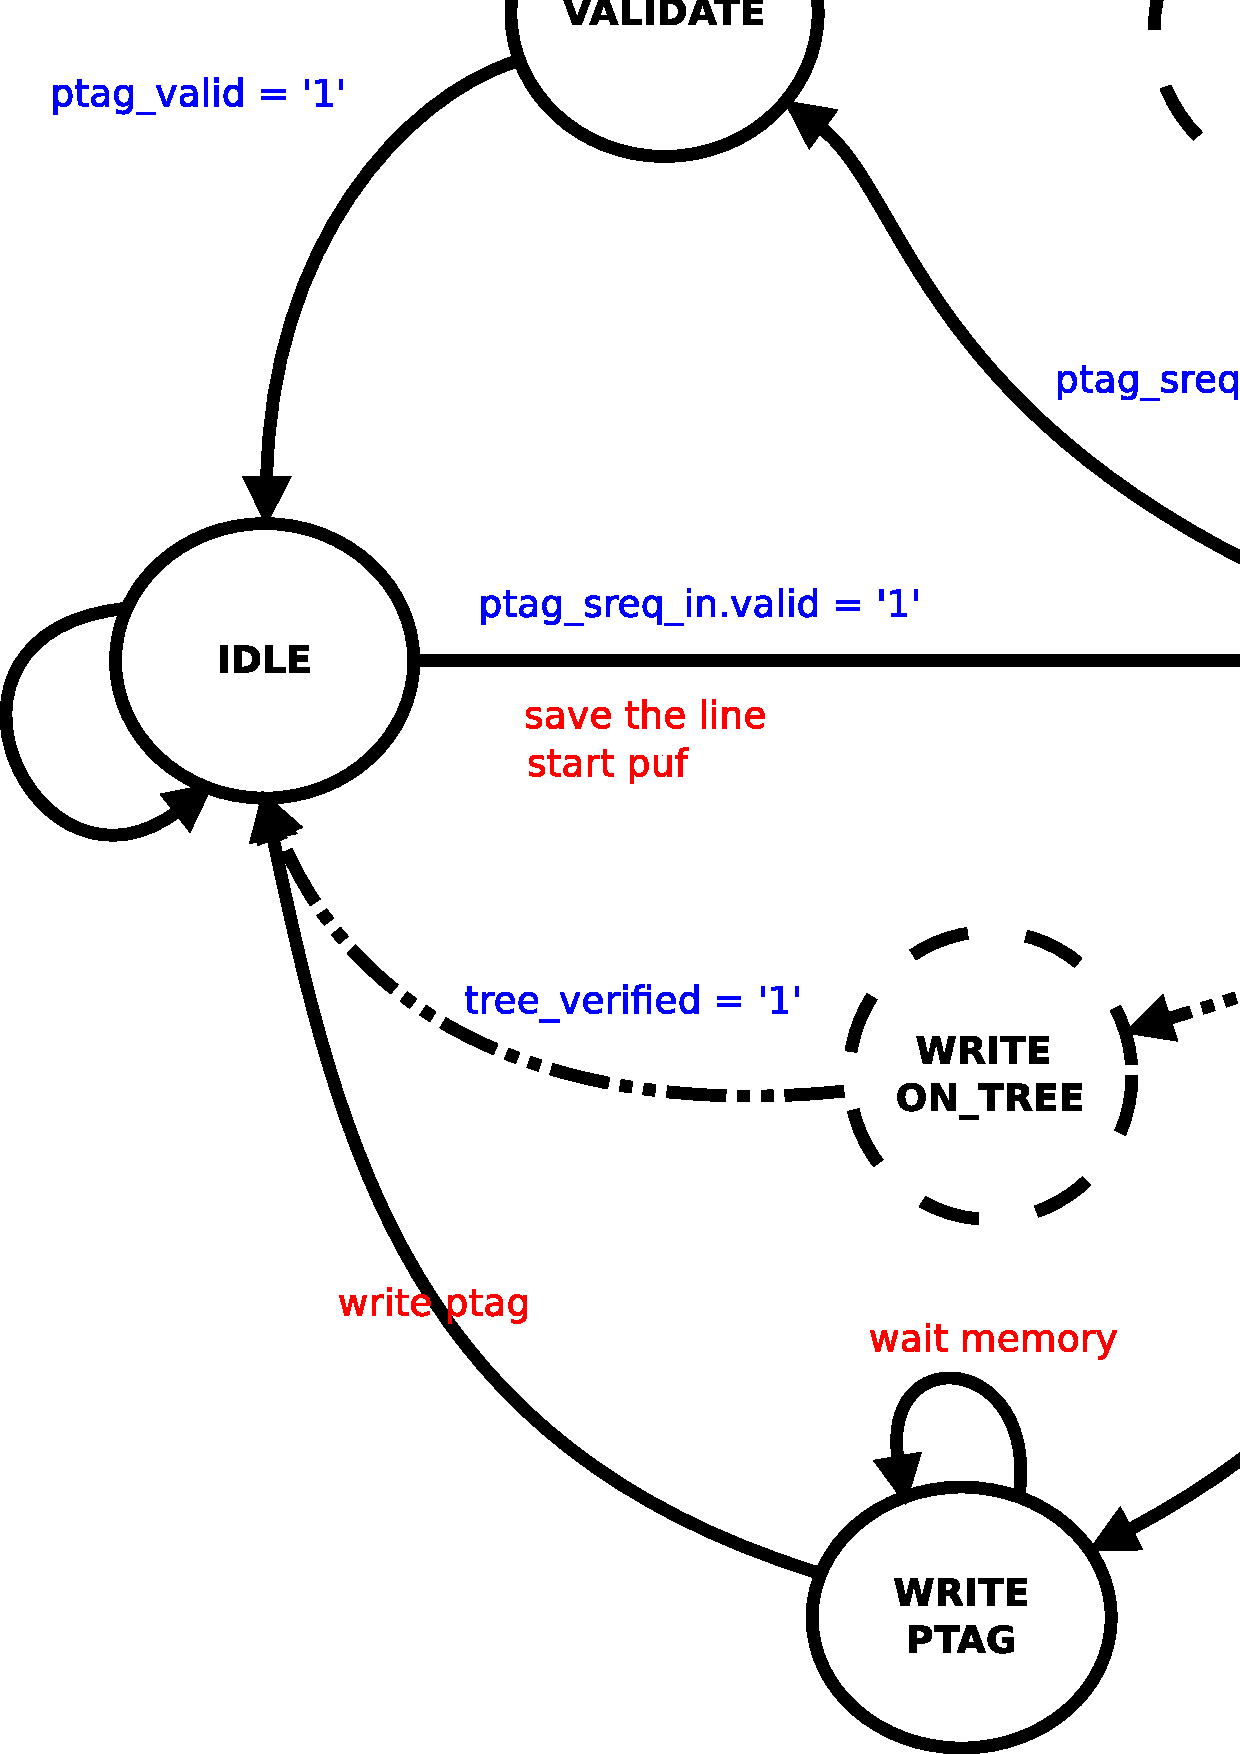
\includegraphics[width=0.70\textwidth]{figures/pdf/sec_engine_sm.pdf}
    \caption{Top of the system  }
    \label{fig:sesm}
\end{figure}


The functional operation of this block consists in two basic actions, given a challenge
calculate the PTAG  using the internal PUF  and if this is a check operation the compare
 the calculated value with the equivalent from the PTAG memory, if its a write operations
 than just store the calculated value in the PTAG memory.the state machine needed to complete
 this task is described bellow.

\begin{itemize}
  \item{\textbf{IDLE}}
 
The security engine stays in  IDLe  until a valid challenge is signalized, then the input is 
registered and a request for the PUF is sent to calculate tha PTAG , as well as read operation 
 to the PTAG memory  in case of a check operation.
 
  \item{\textbf{CALC PTAG}}
  When  a new challenge comes to be checked or written, a new ptag is calculated using the internal PUF, 
  after the calculation is ready the controller goes either to VALIDATE state if this is a check operation
  or to WRITE PTAg state if this is a write operation.
  

  \item{\textbf{VALIDATE}}
  Since in this state the PTAG from the PTAG memory and the calculated from the PUF are ready this state compares
  the values and send the result as a security response to the security handler. Then  the system goes back to IDLE.
  

 \item{\textbf{WRITE PTAG}}
 This state  uses the memory interface to  write the calculated PTAG in the PTAG memory and send a confirmation
 through the security response to the security handler.



\end{itemize}


%===========================================================================================================================================================




\subsection{\ptag~ Memory Management Unit (\pmmu)}
\label{subsec:pmmu}
The \ptag~Memory Management Unit (\pmmu). The main functions of the \pmmu~are to store and request \ptags~from the \ptagmem~and also to decode internal addresses of \ptags~to physical addresses of \ptagmem. In addition to that, \pmmu~can have two distinct designs. If a designer chooses to use timestamps as solution for replay attacks, \pmmu~will have an internal memory to store and control timestamps of the memory blocks. However, if the solution for replay attacks is a \mt\cite{Elbaz2009}, \pmmu~will control verification and update of the tree, as well as it will have a cache memory, the \ptagcache, to speed up these tasks.
\subsubsection{\ptagmem}
\label{subsubsec:ptagmem}
\augusto{describe memories connected to  PMMU}


\section{Operation Modes}
\label{sec:opmodes}

%describe all


\subsection{Runtime Phase}
\label{subsec:runtimephase}
\def\fenroll{Figure \ref{fig:fuzzy-extractor} \subref{fig:fuzzy-enroll}}
\def\fregen{Figure \ref{fig:fuzzy-extractor} \subref{fig:fuzzy-regen}}
After the enrollment phase, \cshia~instances are ready for distribution.Here is how \cshia's components work together. \handler~checks for memory read-write operations of the processor. When it perceives a memory read it will capture memory words \andor~request memory words to compose a memory block. Then it sends this memory block and its address to \seceng. On its turn, \seceng~uses \pmmu~to bring the corresponding \ptag~of that memory block from \ptagmem, while \ptaggen~computes a \ptag~using the content served by \handler. After that, the \ptag~brought from \ptagmem~and the one computed are compared. If they match, \seceng~knows that neither the \ptag~nor the memory block were tampered with. Otherwise, \seceng~alerts the handler that can isolate the processor or sends a non-maskable interrupt to the processor.


For write operations, the process is simpler. Once any memory block that reached the processor was verified for integrity and authenticity, \handler~can serve the cache line to \seceng~that uses \ptaggen~to compute a new \ptag~and \pmmu~sends that \ptag~to \ptagmem.  During the product lifetime, the device can be rebooted and turned off and on multiple times. While this will not affect \ptags, which are externally stored in \ptagmem, the secret key has to be recovered every time the system comes back from off-line periods. This recovery procedure of the \fuzzy~is described next.

\subsubsection{Key Regeneration}
\label{subsubsec:Key-Regenation}
\begin{figure}[!t]
	\centering
	\includegraphics[width=0.7\textwidth]{key-construction}
% 	\includegraphics[scale=0.325]{key-construction}
	\caption{Key generation on \cshia.}
	\label{fig:key-construction}
\end{figure}

During the enrollment there were 8 challenges selected to produce four $r_i$ and four $w_i$ values. These challenges and helper data can be exposed off-chip and stored in \ptag~Memory if the designer chooses to do so. The recovery process of the secret key can be seen in \fregen. After using the challenges and all helper data, the syndromes are recovered. Due to inconsistent nature of \pufs, the fuzzy extractor actually recovers bit-flipped versions $w'_i$ and $r'_i$, what leads to the \bch~decoder receive $r'$ and $s'$. Once bit flips in $r_i$ values are corrected, the \fe~uses all $r_i$ to regenerate the secret key as Figure \ref{fig:key-construction} shows.

\subsection{Enrollment Phase}
\label{subsec:Enrollment-Phase}

In order to ensure authenticity and integrity, an initial procedure has to be conducted by the manufacturer\slash{}vendor. This enrollment procedure will activate the \fuzzy~to extract the secret key from \pufs. Once that is done, the \handler~brings all memory blocks for tag generation. Next, we detail this procedure.

\subsubsection{Key Extraction}
\label{subsubsec:Key-Extraction}

\ptag~Generator implements a Pseudo-Random Function (\prf), which is a primitive cryptographic very similar to a hash function with an important difference: the input processing is based on a secret key. In order to provide uniqueness to every \cshia~instance this key has to be unique. As aforementioned, \pufs~cannot be cloned, thus they can provide this uniqueness. Nevertheless, one big conundrum of using electronic \pufs~to generate keys is that they are inherently unstable. Due to their nature of leveraging on imperfection of the fabrication process, external factors such as temperature variation, voltage variation, etc., can interfere on their responses. Thus, varying responses to challenges during the lifetime of devices. In order to provide consistence in \puf~responses, \fuzzy~(\fe) are employed. In simple terms, \fes~are schemes comprised of an extraction algorithm and a recovery procedure. Becker provides a solid review and formal definitions in \cite{Becker2017:RobustFuzzyExtractor}.

There are multiple ways of implementing a \fuzzy. Originally, \cshia~was proposed using a Code-offset \fe, which is well-known to reduce entropy of extracted keys \cite{Armknecht2011:Formalization}. To strengthen the \cshia~design, we now use an adapted version of the Index-based Syndrome (\ibs) \fe~proposed by Yu and Devadas in \cite{Yu2010:RobustErrorCorrection}. \fenroll~illustrates the process of key extraction of \cshia's \fe. In general terms, a bit string $r$ is extracted from \pufs. Then, the \fe~generates a syndrome $s$ of $r$ using a $(n,k,t)$ Error Correction Code (\ecc). The \fe~also extracts a bit string $w$ and combines it to the syndrome $s$ to generate an encoded helper data $h$. This helper data $h$ can be externally exposed and will not leak information about $r$ (that can be used as secret key or derive the key).


\begin{figure}
     \centering
     \begin{subfigure}[b]{0.5\textwidth}
         \centering
         \includegraphics[width=\textwidth]{fuzzy-enroll}
         \caption{\fuzzy~during key extraction.}
         \label{fig:fuzzy-enroll}
     \end{subfigure}
     \hfill
     \begin{subfigure}[b]{0.5\textwidth}
         \centering
         \includegraphics[width=\textwidth]{fuzzy-regen}
         \caption{\fuzzy~during key regeneration.}
         \label{fig:fuzzy-regen}
     \end{subfigure}

        \caption{\fuzzy~actions during the enrollment and recovery procedure.}
        \label{fig:fuzzy-extractor}
\end{figure}

To fully explain \fenroll, the chosen parameters are detailed. First, \cshia~incorporates \pufs~that produce 64-bit responses (more details in the next section). These \pufs~will be responsible to generate each string $r$ and $w$ that are 64 bits long. To match the length of $r$ and $w$, \cshia~has a $(127, 64, 10)$-\bch~\ecc. As \fenroll~depicts, there are four bit strings $r_i$, which are compounded two by two and fed to the \prf~(Figure \ref{fig:key-construction}). Such combinations were specifically designed to match the \prf~chosen for \cshia, the \siphash~\cite{Aumasson2012:SipHash}, which has an output of 64 bits and uses key of 128 bits. Therefore, the first pair of bit strings $r_i$ is concatenated with a constant and processed by the \prf~using the second pair of bit string $r_i$ as key. That generates a hash $K_1$. Then, inverting their places and concatenating the second pair with a different constant, a hash $K_2$ is obtained. Concatenating $K_1$ with $K_2$ results in $K$ which is the secret key of \cshia. Notice that $C_1$ and $C_2$ in Figure \ref{fig:key-construction} are replacing addresses for input of the \ptaggen. Further details of security will be given in the following sections, however, one can notice that assuming that each bit string $r_i$ has at least half of their length of entropy, each part of the key will have full entropy. Hence, the key has full entropy. 

\subsubsection{Full Memory Protection}
\label{subsubsec:Full-Memory-Protection}

The Enrollment Phase proceeds to tag the memory range the manufacturer\slash{}vendor specified during design. Now that \ptaggen~has an unique key, \seceng~orders \handler~to bring all memory blocks and deliver them to it. \seceng~will use \ptaggen~to generate \ptags, however, depending on the solution against replay attacks a designer chooses, \ptaggen~is used differently. 

% \paragraph{Timestamps Generation}
% \label{paragraph:Timestamps-Generation}

% When timestamps are the solution against replay attacks, \pmmu~will have a timestamp memory. This timestamp memory has the depth of the number of data memory blocks the designer chose to cover. Thus, before \handler~hands in data memory blocks, \pmmu~will clear the entire timestamp memory to avoid uninitialized values. While \seceng~receives code memory blocks, generated \ptags~are just passed to \pmmu~that stores them in \ptagmem. As \handler~starts to pass data memory blocks to \seceng, \pmmu~increments the timestamp of each memory block received and passes this value to \seceng, which combines with the address of the memory block. This combination is then concatenated with the memory block and then finally hashed into a \ptag. \pmmu~receives this \ptag~and stores it in \ptagmem.

% \paragraph{\mt~Generation}
% \label{paragraph:Merkle-Tree-Generation}

% A \mt~solution is more complex. The first procedure is very straightforward. \seceng~receives memory blocks and their addresses from \handler~and uses \ptaggen~to generate \ptags. \pmmu~receives these \ptags~and sends them to \ptagmem. After all memory blocks had their \ptags~generated, \pmmu~starts to bring \ptags~of data memory blocks. As soon as a chunk of \ptags~is formed, a \ptag~internal address of the chunk is calculated. \pmmu~provides this internal address and the chunk to \ptaggen~that generates a \ptag. This \ptag~is returned to \pmmu~that stores it in \ptagmem. This process will continuously happen (as we can see in Figure \ref{fig:vtree}) until \pmmu~identify that the last \ptag~calculated has no siblings. Hence, it is the root \ptag, which must be stored inside \pmmu. It is worth to clarify that \ptag~internal address is an address space that facilitates computation and identification of descendants and ancestors. Each internal address is directly translated to a physical address by \pmmu~and this translation has as goal to minimize unused spaces in \ptagmem. Moreover, in terms of security, this internal address mitigates a very specific attack on the tree, in which an descendant has the same \ptag~as one of its ancestors. In this case, an attacker could try to perform a relocation attack likewise. 


\chapter{CSHIA  Prototype}
\label{chap:cshia_prototype}
To test the \cshia~ architecture  we utilized industry standard IPs provided with no cost for academic purposes, the target processor to receive the security updates was the Leon3, any processor with an AMBA2 interface  could be used since the goal of this work is to test how easy the implementation fits an already existing design and  the impact on the performance. This chapter shows the prototype hardware setup and the tools used to make it work.

\section{Hardware setup}
\label{sec:hardware_setup}

We chose the \leon~platform from Cobham Gaisler~\cite{Leon} to implement \cshia. \leon~is a \vhdl~implementation of a SPARC V8 processor with configurable parameters, which together with some additional IP cores provide a suitable solution for embedded systems. In addition, \leon~has a free version for academic purposes that include sophisticated debugging tools, and it is available for a variety of \fpga~Development kits. Gaisler keeps an email list for support and constant updates are provided. All these features are interesting because \cshia~can be an extension of the platform available to the research community, and which also has solid design choices since \leon~is a product available to the industry.

The implementation is based on Figure \ref{fig:cshia}. \leon's processor (the core) is connected through the main memory by a \amba~Bus version 2.0. In our modification, the processor's \io~master bus connects it to \handler, which then provides a new \io~master bus for the rest of the components in the platform. Thus, \handler~is transparent to all components of the platform, even the core. One of the components that is specific of \leon's platform is the Debug Support Unit (\dsu), which allows a designer using a debug host (such as a computer) to connect to development kits running \leon. Through the debugging connection, a program can be loaded to the \fpga~memory, started, paused, among other useful functions.

We implemented \cshia~in an Altera \fpga~Development Kit DE2-115. The parameters of the processor and \cshia~are in Table \ref{tab:config}. The Altera's kit allows the processor to run at 50 MHz. The total amount of SDRAM memory dedicated to \leon~is 128 MB. As convention all programs starts by its \texttt{.text} segment (code) at the address \texttt{0x40000000}. We set \texttt{.data} segment (data) to start at \texttt{0x40013000}, or at \texttt{0x40023000}, depending on the size of the code segment. As described in the previous section, \handler~has a buffer that stores memory words. When these words form a memory block, it is handed to \seceng. We set the size of this buffer to 4 cache lines, which gives a total of 128 bytes. The 128-bit \siphash's key is extracted from 64 Arbiter \pufs~(\apufs). Although any \puf~could be used, due to the simplicity of design we chose the \apuf~as a proof of concept. Each \apuf~has a 64-bit challenge input. \ptag~generation lasts 10 cycles, between \seceng~request and \ptaggen~reply.

\begin{table}[!t]
  \center
  \caption{\cshia~\fpga~implementation configuration.} 
  \label{tab:config}
  \footnotesize
  \begin{tabular}{|l|l|}
%\    \noalign{\hrule height 1pt}
%\    \rowcolor{lightgray}
    \hline
      Component & Parameter\\ 
    %\noalign{\hrule height 0.75pt}
    \hline
    \hline
      \leon~Processor & \\
      \hspace{0.25in} Frequency & 50 MHz\\
      \hspace{0.25in} Instruction Cache & 16 KB\\
      \hspace{0.25in} Data Cache & 16 KB\\
      \hspace{0.25in} Cache Line Size & 256 bits\\
      \hspace{0.25in} Memory Word & 32 bits\\
    \hline
      Code and Data Memory & Up to 128 MB\\
      \hspace{0.25in} Code Start Address & \texttt{0x40000000}\\
      \hspace{0.25in} Data Start Address 1 & \texttt{0x40013000}\\
      \hspace{0.25in} Data Start Address 2 & \texttt{0x40023000}\\
    \hline
      \handler~Buffer & 128 Bytes\\
    \hline
      \fuzzy & \\
      \hspace{0.25in} \ecc & (127,64,10)-\bch\\
      \hspace{0.25in} \pufs & 64 $\times$ 64-bit Arbiter \pufs\\
    \hline
      \ptaggen & \\
      \hspace{0.25in} \prf & \siphash-2-4\\
      \hspace{0.25in} \siphash-2-4 key & 128 bits\\
      \hspace{0.25in} \ptag~generation & 10 cycles\\
      \hspace{0.25in} \ptag~length & 64 bits\\
    \hline
      \ptag~Memory & 216,064 bytes\\
      \hspace{0.25in} Code and Data \ptags & 18816 words of 64 bits\\ 
      \hspace{0.25in} \mt~\ptags & 8192 words of 64 bits\\ 
      \hspace{0.25in} Data coverage & 512 KB\\
      \hspace{0.25in} Total coverage & 588 KB\\
    \hline
      \pmmu & \\
      \hspace{0.25in} Time Stamp Memory & $2^{14}$ timestamps\\
      \hspace{0.25in} Time Stamp Length & 16 bits\\
      \hspace{0.25in} \ptag~Cache & 4 KB \\
      \hspace{0.25in} \pmmu~Buffer for \mt & 2 * number of cache lines\\
    \hline
  \end{tabular}
%\vspace*{-12pt}
\end{table}

Continuing to look at Table \ref{tab:config}, the \ptagmem~uses internal memory of the \fpga. This option arose due to limiting options available in the kit. Because we wanted to design a 64-bit bus memory, no better option than internal memory was available. The \sram~of the kit only allowed 16-bit words. We also could not increase the frequency of the \sram~using PLLs since its maximum frequency was limited to 125 MHz, and, to simulate a 64-bit bandwidth, we would need at least a \sram~operating at 200 MHz. The option for \fpga~internal memory limited our coverage to a maximum of 512 KB of data memory, which resulted in a memory overhead of 36 \% (code, data, and \mt). In addition, to reduce unused memory words in \ptagmem, we split it into two. This allowed to create an easy decoder to separate \ptags~of memory blocks from those of chunks of \ptags. 

%Due to the high utilization of internal memory, timestamp memory became limited to $2^{14}$ 16-bit words to cover the 512 KB of data memory. This represents 5.4\% of the total 588 KB main memory coverage. The \ptagmem~utilization for this solution was up to 147 KB (code and data), or 25\% overhead. Table \ref{tab:config} also shows the \ptag~cache's configuration. Since this cache is an internal memory as well, it was limited to 4 KB. That limitation did not prevent us of evaluating the cache in multiple configurations. We evaluated this cache in different configurations of lines, set associativity, and replacement policies. Finally, as previously discussed, \pmmu~requires a buffer to stall a \ptag~cache write or read while an eviction is required. We calculated that this buffer needs to be at most 2 times the number of lines in \ptagcache. 

%One last information about our \fpga~\cshia~implementation is that it had three modes of operation. In the first mode, called \baseline, the \handler~is disabled and all security-specific hardware is bypassed. A second mode, the \timestamp, activates \pmmu~for timestamps only. Finally, the third mode, \textit{\cshia-MT}, disables timestamps and activates the cache in \pmmu~for supporting the Merkle Tree implementation. Being able to switch between those modes only using switch keys of the development key helped us in debugging and evaluating the performance of the architecture.


\section{GAISLER Tools}
\label{sec:gaisler_tools}
\subsection{Overview}
 GRMON is a general debug monitor for the LEON processor, it includes the following functions:
\begin{itemize}

 \item Read/write access to all system registers and memory
 \item Built-in disassembler and trace buffer management
 \item Downloading and execution of LEON applications
 \item Breakpoint and watchpoint management
 \item Remote connection to GNU debugger (GDB)
 \item Support for USB, JTAG, RS232, PCI, Ethernet and SpaceWire debug links

\end{itemize}

\subsection{Debug}

The GRMON debug monitor is intended to debug system-on-chip (SOC) designs based on the LEON processor. 
The monitor connects to a dedicated debug interface on the target hardware, through which it can perform
read and write cycles on the on-chip bus (AHB).LEON3 also supports JTAG, ethernet and
spacewire (using the GRESB ethernet to spacewire bridge) debug interfaces. On the target system, all debug
interfaces are realized as AHB masters with the debug protocol implemented in hardware. There is thus no
software support necessary to debug a LEON system, and a target system does in fact not even need to have a processor present.

 \begin{figure}[ht]
    \centering
    \includegraphics[width=0.75\textwidth]{figures/others/grmon_ex.png}
    \caption{GRMON  Interface }
    \label{fig:grmon_int}
\end{figure}
GRMON can operate in two modes: command-line mode and GDB mode. In command-line mode, GRMON
commands are entered manually through a terminal window. In GDB mode, GRMON acts as a GDB gateway
and translates the GDB extended-remote protocol to debug commands on the target system.
GRMON is implemented using three functional layers: command layer, debug driver layer, and debug interface
layer. The command layer consist of a general command parser which implements commands that are independent
of the used debug interface or target system. These commands include program downloading and flash
programming.
The debug driver layer implements custom commands which are related to the configuration of the target system. 
GRMON scans the target system at startup, and detects which IP cores are present and how they are con-
figured. For each supported IP core, a debug driver is enabled which implements additional debug commands
for the specific core. Such commands can consist of memory detection routines for memory controllers, or program
debug commands for the LEON processors.
The debug interface layer implements the debug link protocol for each supported debug interface. The protocol
depends on which interface is used, but provides a uniform read/write interface to the upper layers. Which
interface to use for a debug session is specified through command-line options during the start of GRMON.





\chapter{CSHIA  Evaluation}
\label{chap:cshia:evaluation}
\section{Area?Performance?}
\augusto{Are we going to use the same results as Caio ??}

\chapter{Conclusion}
\label{chap:conclusion}
 \pufs~are physical security primitives which enable trust in the context of digital hardware implementations of cryptographic constructions, in particular, they can initiate physically unclonable and secure key generation and storage. In this dissertation, the implementation of \cshia, a platform that utilizes \pufs~to achieve information security objectives that are data integrity and authentication is presented. 

We described in detail the building blocks of this implementation and the way this system can work at block level together with the impact of this implementation in comparison to the non-secure system.

In  Chapter \ref{chap:fundamental_concepts}, we introduced the basics of \pufs~and the information security goals of this work, in order to make clear what we want to achieve. The importance of authentication and integrity was highlighted and examples of \pufs~in order to give useful examples of how they work and fit in the context of this work.

A review of the related work was presented in chapter \ref{chap:related_work}, where similar architectures implemented security features to provide similar features as \cshia, but in this kind of work, it is difficult to have a fair comparison  between  the security features and the implementation details, mostly because of \fpga~limitations and the way synthesis tools deal with different designs. So the characteristics of each work were resumed and compared with strong and weak points to make it easier to see where \cshia~fill the gaps of other works, presenting performance, area, power estimations and now implementations details of the how the security blocks work on hardware.

The \cshia~architecture implementation was described in Chapter \ref{chap:cshia_architecture}, with an extensive description of the AMBA protocol and all the steps required to get the results achieved, the initial \cshia~architecture and which components were added to extend \cshia~to make it more robust and improve integrity. The contributions of this work were described and an in-depth explanation of how the building blocks of this implementation work with timing diagrams and interfaces explained.


Chapter \ref{chap:cshia_prototype} presented the details of the prototype, and how using the Leon3 processor with our tailored security IPs in a DE2-115 \fpga~development kit we could sustain the original 50MHz, and due to the limitations of the kit, we covered 512Kb of memory. The evaluation of the prototype was presented in Chapter \ref{chap:cshia:evaluation}  were we show the selected benchmarks together with the total coverage and performance of the \cshia~extended implementation where without the \mt~the average  performance degradation is $2.76\%$ and with  it goes to $5.77\%$ in exchange of a more robust design. Analyzing area and power the \cshia~logic overhead achieved $34\%$ mostly due to the \sbuf~that scales when accessing big \slines.

  The contributions of this work were submitted to the following venues 
 \begin{itemize}
 \item{TETC-2017} Publication 1  - description 1
 \item{MicPro-2018} Publication 2 - description 2
 \end{itemize}
%\endgroup
% As referências:
\bibliographystyle{plain}
\bibliography{aqueiroz_msc_dissertation}



% Os anexos, se houver, vêm depois das referências:
\appendix
\chapter{Type Description}
\label{ap:signals}

\begin{table}[H]
\centering
\label{table:psrtype}
\begin{tabular}{l l p{55mm}}
\textbf{Signal} & \textbf{Type}      & \textbf{Description}                                         	\\ \hline \hline
cache\_line 	& std\_logic\_vector & the entire cach line                                        	\\ \hline
base\_addr  	& std\_logic\_vector & base physical address of the line                            	\\ \hline
valid       	& std\_logic         & asserted if the line is valid                                	\\ \hline
wr\_ptag    	& std\_logic         & asertedif the calculated ptag will be  writen in th e PTAG mem    \\  \hline
\end{tabular}                                                                                                                                   
\caption{\textbf{ptag\_sec\_req\_type} content description}                                                                                              
\end{table}                                                                                                                                     


\begin{table}[H]
\centering
\label{table:psvtype}
\begin{tabular}{l l p{55mm}}
\textbf{Signal} & \textbf{Type}      & \textbf{Description}                        \\ \hline \hline
ptag 		& std\_logic\_vector & the calculated ptag                         \\ \hline
valid 		& std\_logic         & asserted when  ptag is valid                \\ \hline
line\_secure 	& std\_logic         & asserted if the provided line is secure     \\ \hline
ready 		& std\_logic         & asserted when ready to receive a new line   \\  \hline
\end{tabular}                                                                                                                                   
\caption{\textbf{ptag\_sec\_val\_type} content description}                                                                                              
\end{table}    




\begin{table}[H]
\centering
\label{table:pmrqtype}
\begin{tabular}{l l p{55mm}}
\textbf{Signal} & \textbf{Type}      & \textbf{Description}                     \\ \hline \hline
we      & std\_logic;                 & active high write enable                \\ \hline
address & std\_logic\_vector           & memory address                         \\ \hline
data    & std\_logic\_vector           & data to be writen                      \\ \hline
\end{tabular}                                                                                                                                   
\caption{\textbf{ptag\_mreq\_type} content description}                                                                                              
\end{table}     

\begin{table}[H]
\centering
\label{table:pmrtype}
\begin{tabular}{l l p{55mm}}
\textbf{Signal} & \textbf{Type}      & \textbf{Description}                     \\ \hline \hline
data 		& std\_logic\_vector   & PTAG read from memory                  \\ \hline
 \end{tabular}                                                                                                                                   
\caption{\textbf{ptag\_mresp\_type} content description}                                                                                              
\end{table}    




\begin{table}[H]
\centering
\label{table:abhitype}
\begin{tabular}{l l p{55mm}}
\textbf{Signal} & \textbf{Type}      	& \textbf{Description}                  \\ \hline \hline
    hgrant	& std\_logic\_vector 	& bus grant                             \\ \hline
    hready	& std\_ulogic       	& transfer done                         \\ \hline
    hresp	& std\_logic\_vector	& response type                         \\ \hline
    hrdata	& std\_logic\_vector	& read data bus                         \\  \hline
    hcache	& std\_ulogic       	& cacheable                             \\ \hline
    hirq  	& std\_logic\_vector	& interrupt result bus                  \\ \hline
    testen	& std\_ulogic       	& scan test enable                      \\ \hline
    testrst	& std\_ulogic           & scan test reset          		\\  \hline
    scanen 	& std\_ulogic           & scan enable              		\\ \hline
    testoen 	& std\_ulogic           & test output enable      	 	\\ \hline
 \end{tabular}                                                                                                                         
\caption{\textbf{ahb\_mst\_in\_type} content description}                                                                                      
\end{table}                                                                                             

  
  
  
\begin{table}[H]
\centering
\label{table:ahbotype}
\begin{tabular}{l l p{55mm}}
\textbf{Signal} & \textbf{Type}      & \textbf{Description}                     \\ \hline \hline  

    hbusreq	& std\_ulogic           & bus request                           \\ \hline
    hlock	& std\_ulogic           & lock request                          \\ \hline
    htrans	& std\_logic\_vector	& transfer type                          \\  \hline
    haddr	& std\_logic\_vector 	& address bus (byte)                    \\ \hline
    hwrite	& std\_ulogic           & read/write                            \\ \hline
    hsize	& std\_logic\_vector	& transfer size                         \\ \hline
    hburst	& std\_logic\_vector	& burst type                             \\  \hline
    hprot	& std\_logic\_vector	& protection control                     \\ \hline
    hwdata	& std\_logic\_vector 	& write data bus                         \\ \hline
    hirq   	& std\_logic\_vector	& interrupt bus                          \\ \hline
    hconfig 	& ahb\_config\_type	& memory access reg.                    \\  \hline
    hindex  	& integer  		& diagnostic use only                   \\ \hline
 \end{tabular}                                                                                                                                 
\caption{\textbf{ahb\_mst\_out\_type} content description}                                                                                            
\end{table}                                                                                               



%     \chapter{The grid application generator}
    \ldots

% \appendix
% \chapter{Type Description}
\label{ap:signals}

\begin{table}[H]
\centering
\label{table:psrtype}
\begin{tabular}{l l p{55mm}}
\textbf{Signal} & \textbf{Type}      & \textbf{Description}                                         	\\ \hline \hline
cache\_line 	& std\_logic\_vector & the entire cach line                                        	\\ \hline
base\_addr  	& std\_logic\_vector & base physical address of the line                            	\\ \hline
valid       	& std\_logic         & asserted if the line is valid                                	\\ \hline
wr\_ptag    	& std\_logic         & asertedif the calculated ptag will be  writen in th e PTAG mem    \\  \hline
\end{tabular}                                                                                                                                   
\caption{\textbf{ptag\_sec\_req\_type} content description}                                                                                              
\end{table}                                                                                                                                     


\begin{table}[H]
\centering
\label{table:psvtype}
\begin{tabular}{l l p{55mm}}
\textbf{Signal} & \textbf{Type}      & \textbf{Description}                        \\ \hline \hline
ptag 		& std\_logic\_vector & the calculated ptag                         \\ \hline
valid 		& std\_logic         & asserted when  ptag is valid                \\ \hline
line\_secure 	& std\_logic         & asserted if the provided line is secure     \\ \hline
ready 		& std\_logic         & asserted when ready to receive a new line   \\  \hline
\end{tabular}                                                                                                                                   
\caption{\textbf{ptag\_sec\_val\_type} content description}                                                                                              
\end{table}    




\begin{table}[H]
\centering
\label{table:pmrqtype}
\begin{tabular}{l l p{55mm}}
\textbf{Signal} & \textbf{Type}      & \textbf{Description}                     \\ \hline \hline
we      & std\_logic;                 & active high write enable                \\ \hline
address & std\_logic\_vector           & memory address                         \\ \hline
data    & std\_logic\_vector           & data to be writen                      \\ \hline
\end{tabular}                                                                                                                                   
\caption{\textbf{ptag\_mreq\_type} content description}                                                                                              
\end{table}     

\begin{table}[H]
\centering
\label{table:pmrtype}
\begin{tabular}{l l p{55mm}}
\textbf{Signal} & \textbf{Type}      & \textbf{Description}                     \\ \hline \hline
data 		& std\_logic\_vector   & PTAG read from memory                  \\ \hline
 \end{tabular}                                                                                                                                   
\caption{\textbf{ptag\_mresp\_type} content description}                                                                                              
\end{table}    




\begin{table}[H]
\centering
\label{table:abhitype}
\begin{tabular}{l l p{55mm}}
\textbf{Signal} & \textbf{Type}      	& \textbf{Description}                  \\ \hline \hline
    hgrant	& std\_logic\_vector 	& bus grant                             \\ \hline
    hready	& std\_ulogic       	& transfer done                         \\ \hline
    hresp	& std\_logic\_vector	& response type                         \\ \hline
    hrdata	& std\_logic\_vector	& read data bus                         \\  \hline
    hcache	& std\_ulogic       	& cacheable                             \\ \hline
    hirq  	& std\_logic\_vector	& interrupt result bus                  \\ \hline
    testen	& std\_ulogic       	& scan test enable                      \\ \hline
    testrst	& std\_ulogic           & scan test reset          		\\  \hline
    scanen 	& std\_ulogic           & scan enable              		\\ \hline
    testoen 	& std\_ulogic           & test output enable      	 	\\ \hline
 \end{tabular}                                                                                                                         
\caption{\textbf{ahb\_mst\_in\_type} content description}                                                                                      
\end{table}                                                                                             

  
  
  
\begin{table}[H]
\centering
\label{table:ahbotype}
\begin{tabular}{l l p{55mm}}
\textbf{Signal} & \textbf{Type}      & \textbf{Description}                     \\ \hline \hline  

    hbusreq	& std\_ulogic           & bus request                           \\ \hline
    hlock	& std\_ulogic           & lock request                          \\ \hline
    htrans	& std\_logic\_vector	& transfer type                          \\  \hline
    haddr	& std\_logic\_vector 	& address bus (byte)                    \\ \hline
    hwrite	& std\_ulogic           & read/write                            \\ \hline
    hsize	& std\_logic\_vector	& transfer size                         \\ \hline
    hburst	& std\_logic\_vector	& burst type                             \\  \hline
    hprot	& std\_logic\_vector	& protection control                     \\ \hline
    hwdata	& std\_logic\_vector 	& write data bus                         \\ \hline
    hirq   	& std\_logic\_vector	& interrupt bus                          \\ \hline
    hconfig 	& ahb\_config\_type	& memory access reg.                    \\  \hline
    hindex  	& integer  		& diagnostic use only                   \\ \hline
 \end{tabular}                                                                                                                                 
\caption{\textbf{ahb\_mst\_out\_type} content description}                                                                                            
\end{table}                                                                                               



\end{document}
